\documentclass[12pt,t]{beamer}
\usepackage{hyperref}
\usepackage{localbeamer}
\usepackage{amsmath,amssymb}
\usepackage[all]{xy}
\graphicspath{{./figures/}}

%\newtheorem{definition}{Definition}
%\newtheorem{example}{Example}
%\newtheorem{theorem}{Theorem}
%\newtheorem{lemma}{Lemma}
\DeclareMathOperator{\erf}{erf} \DeclareMathOperator{\prob}{Prob}


\begin{document}

\title[Optimal Microfluidic Mixing and Cutoff]{Cutoffs in Chaotic Map Mixing and \\Topology Optimization of Microfluidic Channels}
\author{Tzu-Chen Liang}
\institute[Stanford University]%
{Aeronautics and Astronautics, Stanford University\\
\url{http://www.stanford.edu/~tzuchen/}} \coauthor{Advised by Matthew West}
\date{December 6, 2007}
\frame{\titlepage}


%%%%%%%%%%%%%%%%%%%%%%%%%%%%%%%%%%%%%%%%%%%%%%%%%%

\begin{frame}
\myframetitle{The Map Defined by Streamlines}
\begin{tabular}{rl}
\includegraphics[width=0.45\textwidth,trim=1cm 1cm 0cm 0cm]{computedmixingchannel}&
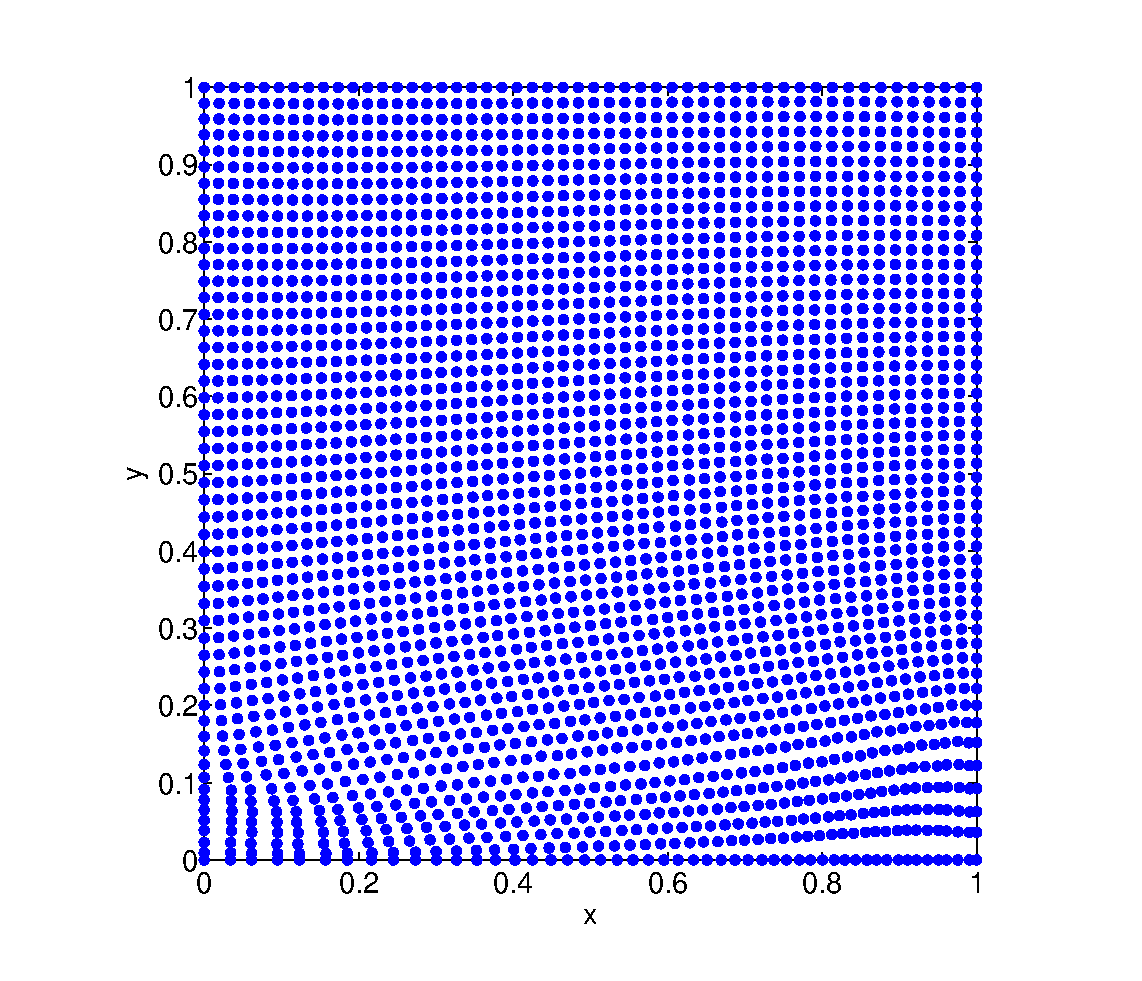
\includegraphics[width=0.45\textwidth,trim=1cm 1cm 0cm 0cm]{mappedpoints}
\end{tabular}
\end{frame}
%%%%%%%%%%%%%%%%%%%%%%%%%%%%%%%%%%%%%%%%%%%%%%%%%%
\begin{frame}
\myframetitle{An Example}
\begin{example}{\bfseries Maximize the downward velocity at the center of the channel}
  \begin{figure}
    \centerline{
      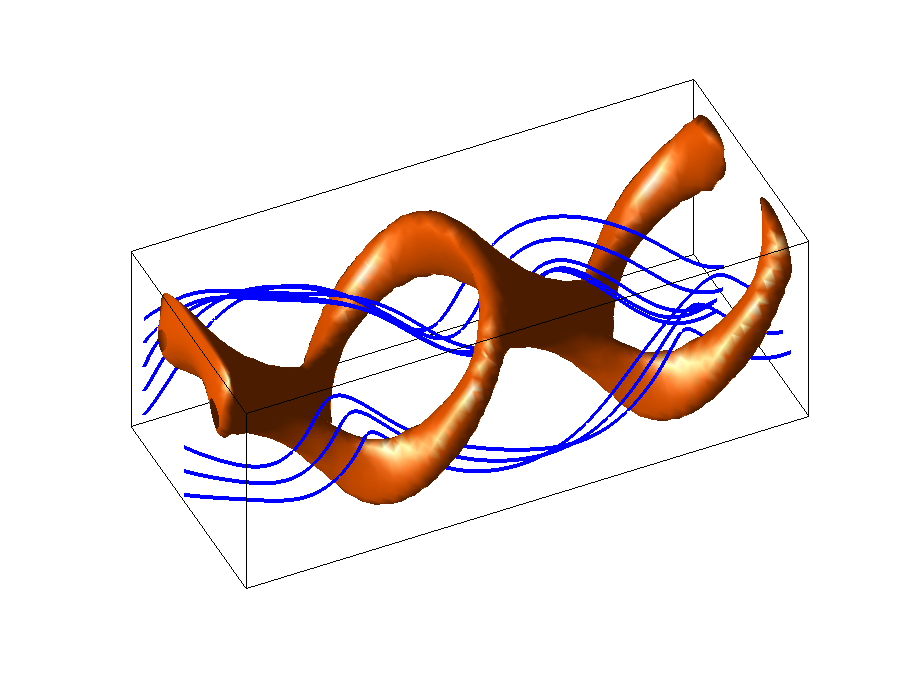
\includegraphics[width=0.45\textwidth]{example1structure2}
       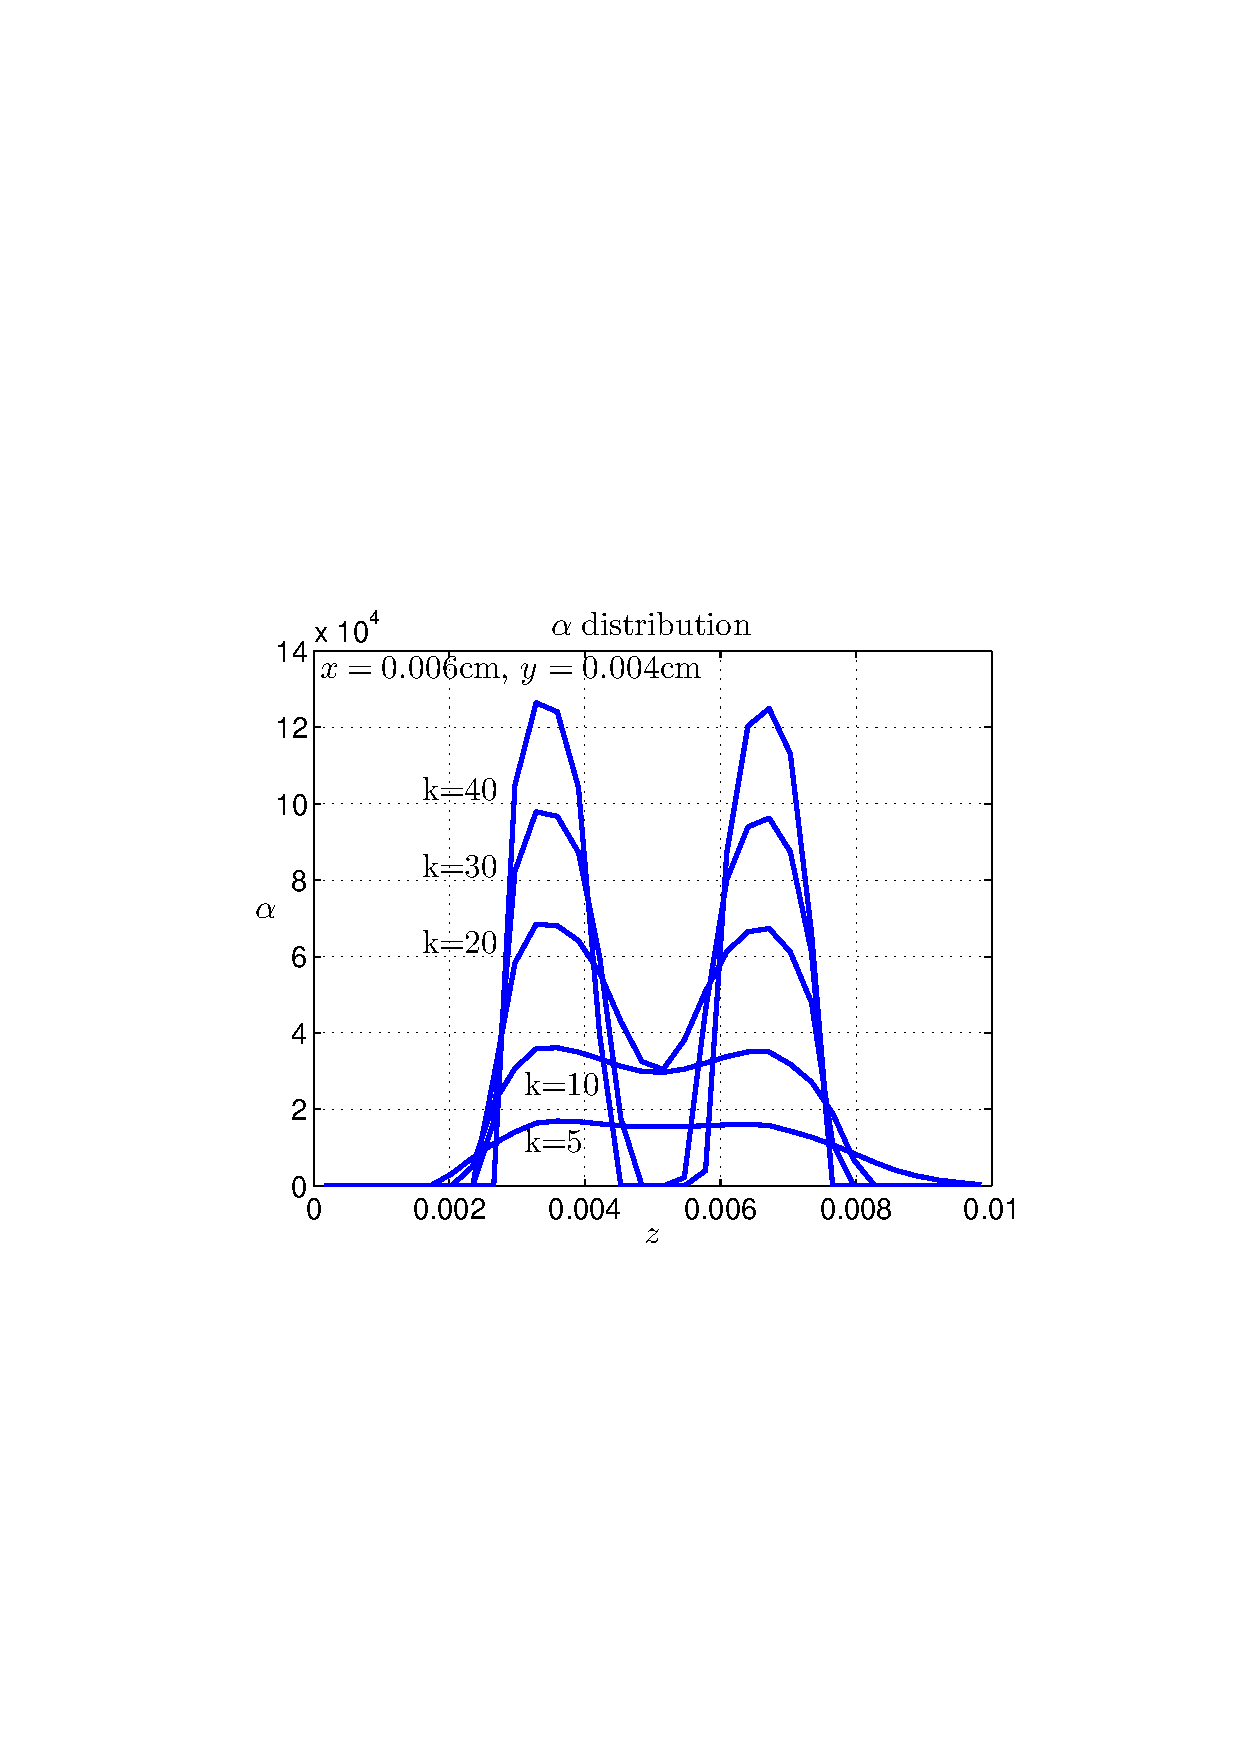
\includegraphics[width=0.45\textwidth]{example1alphaevolve}
    }
  \end{figure}
\end{example}
\end{frame}


%%%%%%%%%%%%%%%%%%%%%%%%%%%%%%%%%%%%%%%%%%%%%%%%%%%

\begin{frame}
\myframetitle{Rotate the Flow $45$ degrees}
%\begin{example}
\begin{tabular}{lr}
 \begin{minipage}[b]{0.5\textwidth}
$S(y,z;y_c,z_c,\theta): (y,z)\mapsto (y_e,z_e)$, and
  \begin{eqnarray*}
     y_e &= y_c + r \cos(\alpha+\theta) \\
     z_e &= z_c + r \sin(\alpha+\theta)
  \end{eqnarray*} 
where $(r,\alpha)=\text{polar}(y,z)$
 
Objective:
 %a flow map to rotate the flow 45 degrees centered at $(0.5,0.5)$ per period of the channel.
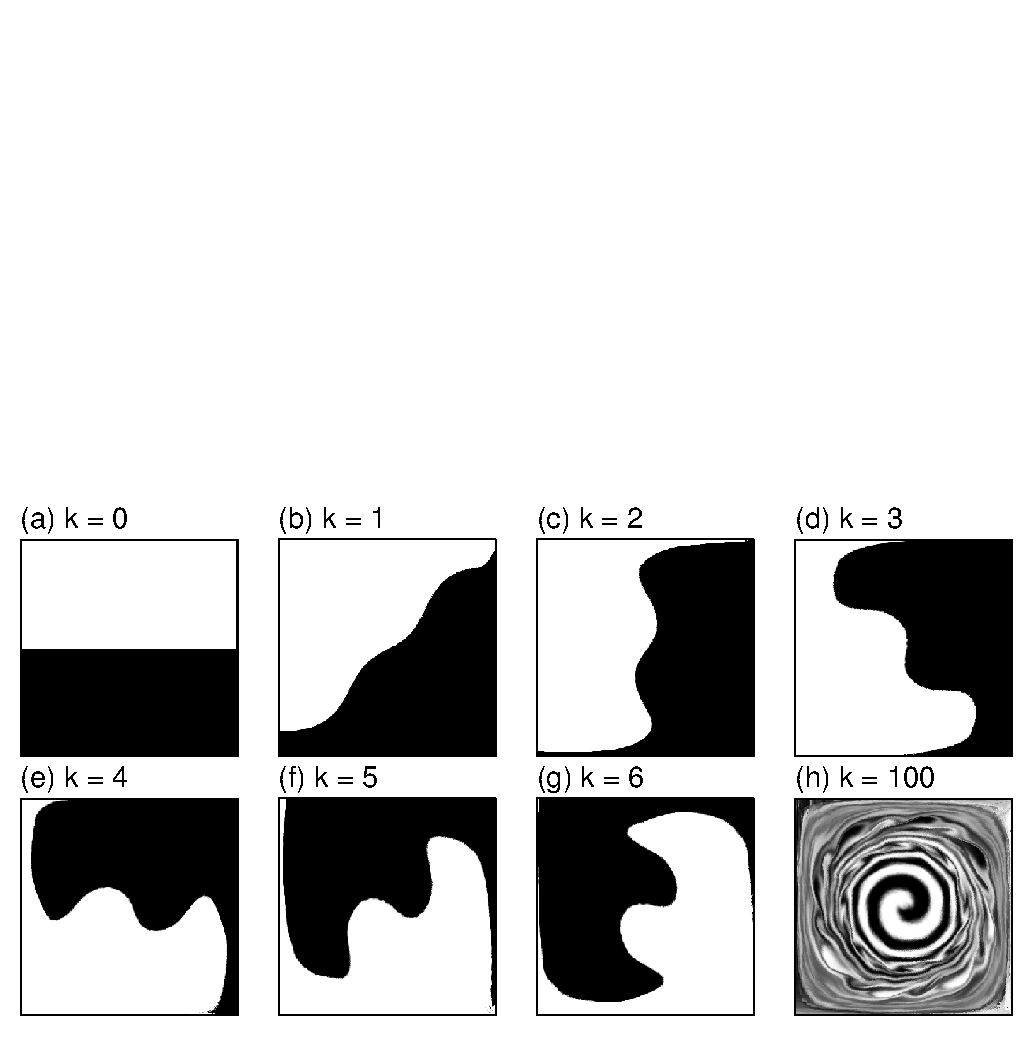
\includegraphics[width=1\textwidth,trim=0cm 0cm 0cm 8cm,clip]{example3simu}
 \end{minipage}
 & \begin{minipage}[b]{6cm}
      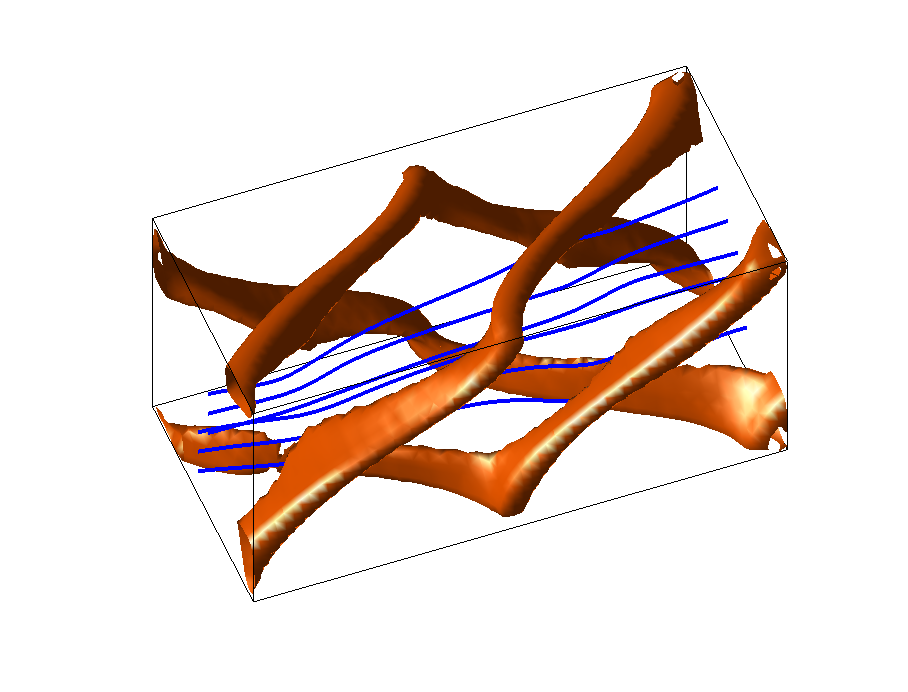
\includegraphics[width=0.8\textwidth,trim=1cm 0cm 1cm 1cm,clip]{example3structure}
      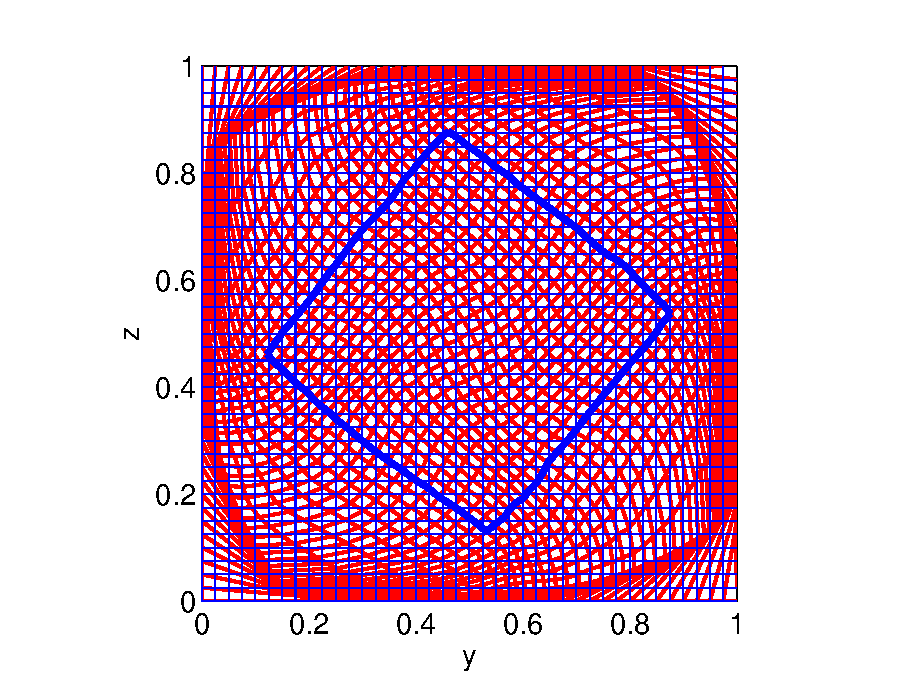
\includegraphics[width=0.8\textwidth,trim=1cm 1cm 1cm 1cm]{example3grid}
 \end{minipage}
\end{tabular}
%\end{example}

\end{frame}

%%%%%%%%%%%%%%%%%%%%%%%%%%%%%%%%%%%%%%%%%%%%%%%%%%%%%%%
%%%%%%%%%%%%%%%%%%%%%%%%%%%%%%%%%%%%%%%%%%%%%%%%%%%%%%%
\begin{frame}
\myframetitle{Simulation versus Experiment}
  \begin{figure}
    \centerline{
       \includegraphics[width=0.6\textwidth]{mixersimu}
       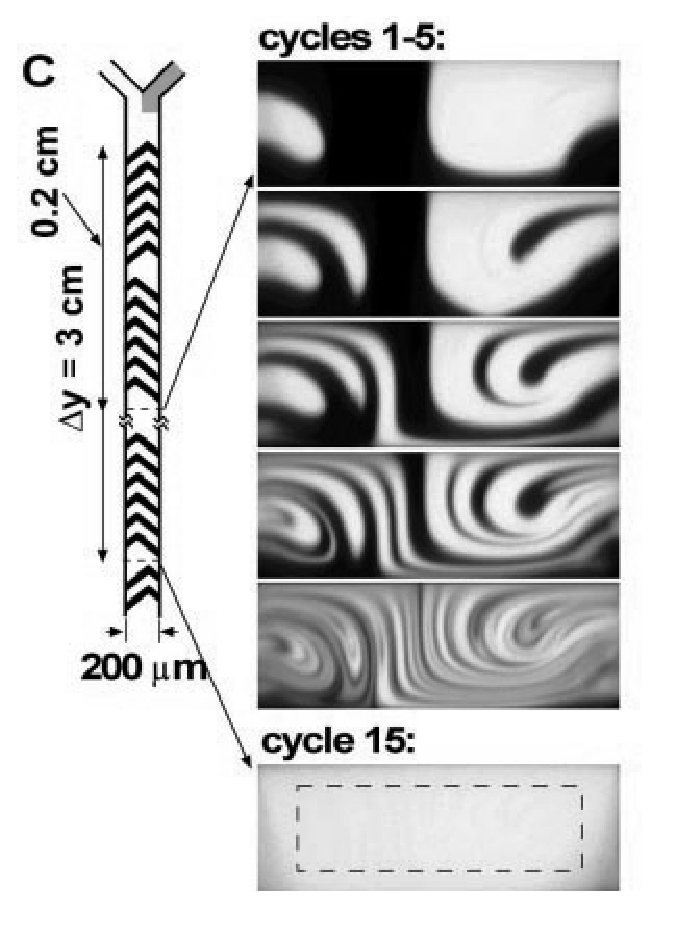
\includegraphics[width=0.4\textwidth]{stroockcrosssection0}
    }
  \end{figure}
\end{frame}

%%%%%%%%%%%%%%%%%%%%%%%%%%%%%%%%%%%%%%%%%%%%%%%%%%%%%%%%%%%%%%%%%%%%%%%%%
%%%%%%%%%%%%%%%%%%%%%%%%%%%%%%%%%%%%%%%%%%%%%%%%%%%%%%%%%%%%%%%%%%%%%%%%%
\begin{frame}
\myframetitle{Cross-sections of the three channels}
  \begin{figure}
    \centerline{
     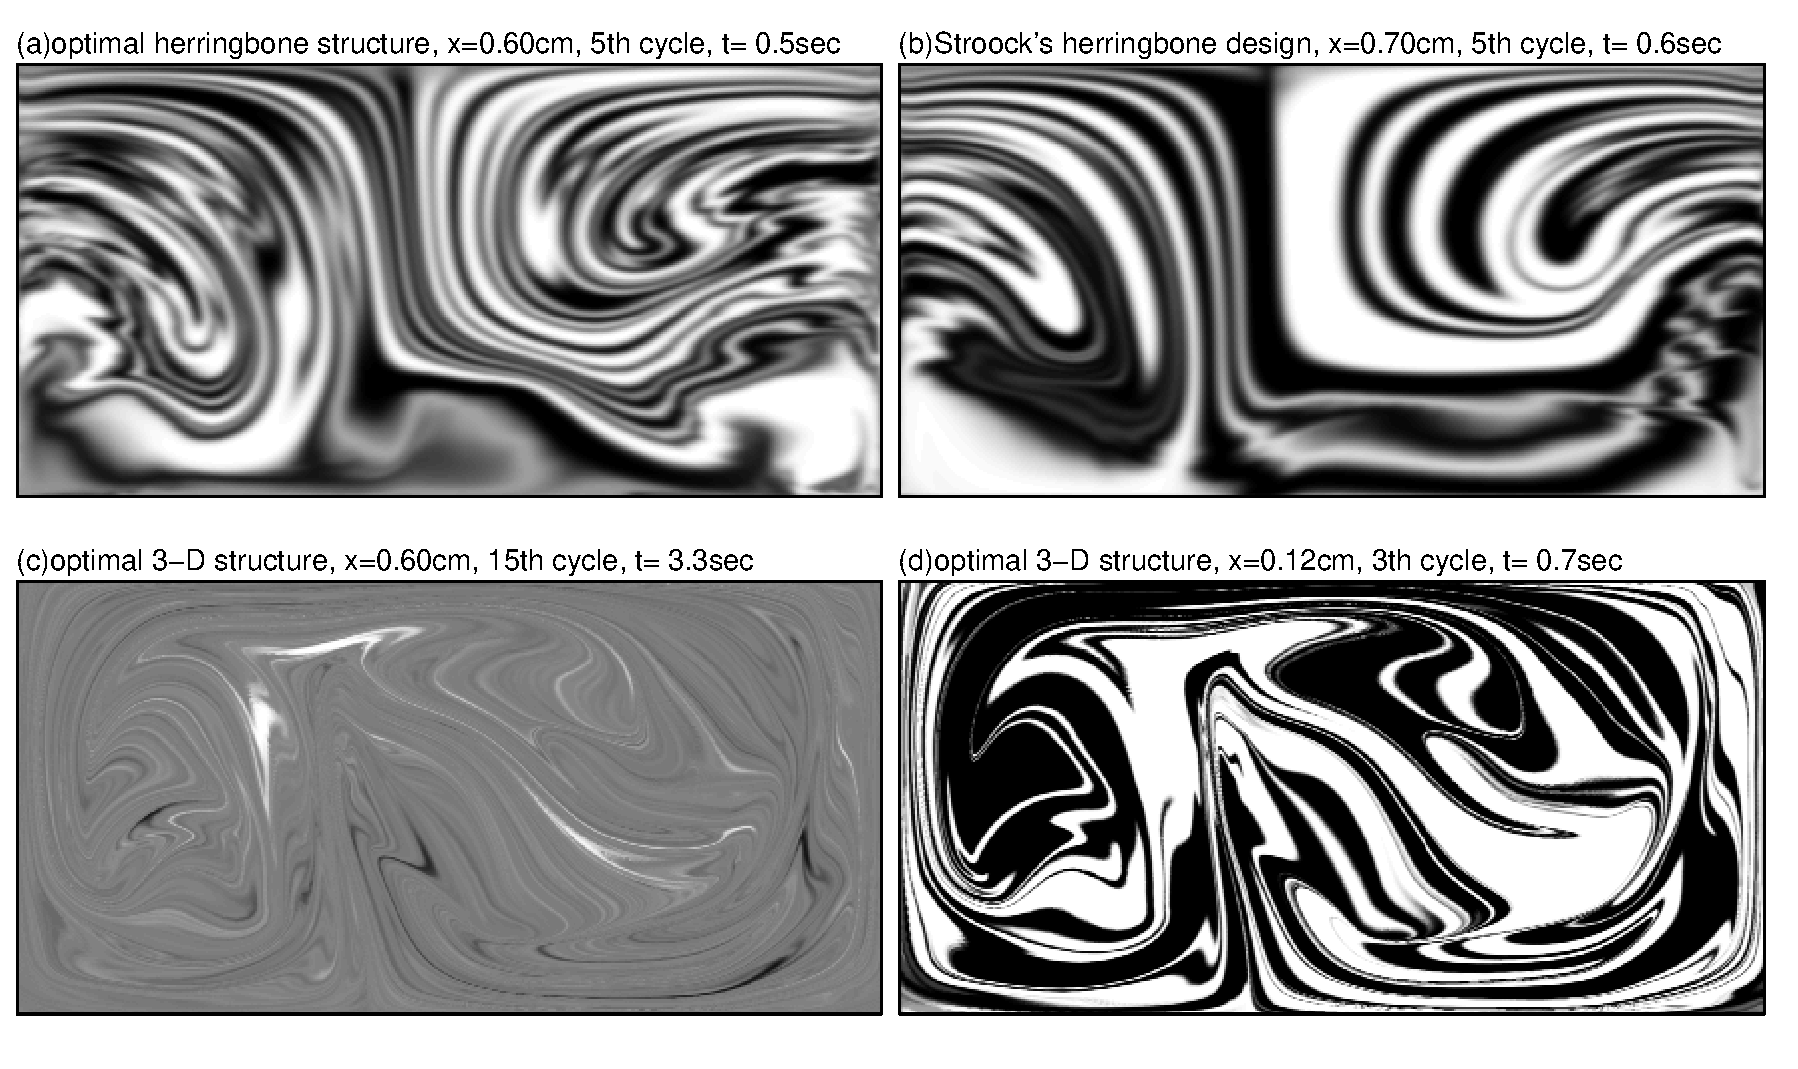
\includegraphics[width=0.8\textwidth]{example2crosscompare}
    }
  \end{figure}
\end{frame}




%%%%%%%%%%%%%%%%%%%%%%%%%%%%%%%%%%%%%%%%%%%%%%%%%%%%%%%%%%%%%%%%%%%%%%%%%
%%%%%%%%%%%%%%%%%%%%%%%%%%%%%%%%%%%%%%%%%%%%%%%%%%%%%%%%%%%%%%%%%%%%%%%%%
\begin{frame}
\myframetitle{Perron-Frobenius Operator and Koopman Operator}
\begin{itemize}
\item Given a map $S:X \rightarrow X$. In the measure space $(X,\mathcal{A},\mu)$,
\item {\bfseries (Perron-Frobenius operator)}
Let $f \in L^1$, for every $A \in \mathcal{A}$ the operator $P:L^1 \rightarrow L^1$ satisfies
  \begin{eqnarray}
    \int_A Pf(x)\mu(dx) = \int_{S^{-1}(A)} f(x)\mu(dx)
  \end{eqnarray}
is the Perron-Frobenius operator associated with $S$.



\item {\bfseries (Koopman operator)}
Let $f \in L^\infty$. The operator $U:L^{\infty} \rightarrow L^{\infty} $ defined by
 \begin{eqnarray}
 Uf(x) = f(S(x))
 \end{eqnarray}
is called the Koopman operator associated with $S$.


\end{itemize}
\end{frame}

%%%%%%%%%%%%%%%%%%%%%%%%%%%%%%%%%%%%%%%%%%%%%%%%%%%%%%%%%%%%%%%%%%%%%%%%%
%%%%%%%%%%%%%%%%%%%%%%%%%%%%%%%%%%%%%%%%%%%%%%%%%%%%%%%%%%%%%%%%%%%%%%%%%
\begin{frame}
\myframetitle{Perron-Frobenius Operator and Koopman Operator}
\begin{itemize}
\item $\mu$: Borel measure. We have
\begin{tabular}{l|rr}
                      & forward in time                    & backward in time     \\
\hline
        probability measure & $P_S$ ,$(A^T)$                       &  $P_{S^{-1}}$ ,$(B^T)$  \\
        function            & $P_{S^{-1}}^* = U_{S^{-1}}$ ,$(B)$ &  $P_S^* = U_S $ ,$(A)$
\end{tabular}

$A,B$ are Markov matrices (Probably infinitely dimensional)

\item $A$ and $B$ have simple relation,
      \begin{eqnarray}
         B = \text{diag}(\bar{\omega}) A^T \text{diag}({\bar{\omega}}^{-1})
       \end{eqnarray}
 where $\bar{\omega}$ is the invariant measure of $S$
\end{itemize}
\end{frame}
%%%%%%%%%%%%%%%%%%%%%%%%%%%%%%%%%%%%%%%%%%%%%%%%%%%%%%%%%%%%%%%%%%%%%%%%%
%%%%%%%%%%%%%%%%%%%%%%%%%%%%%%%%%%%%%%%%%%%%%%%%%%%%%%%%%%%%%%%%%%%%%%%%%

\begin{frame}
\myframetitle{Model Reduction}
\begin{itemize}
\item Consider a finite state space $X =\mathbb{Z}_n$, and a finite observation space $Y=\mathbb{Z}_m$. $n>m$
\begin{eqnarray*}
   P_{ij}&=&\prob\left( X^{k+1}=j| X^k=i \right)\\
   B_{ij}&=&\prob\left( Y^k=j| X^k=i \right)
\end{eqnarray*}
\item the "best" model $\bar{P} \in \mathbb{R}^{m \times m}$ of $P \in \mathbb{R}^{n \times n}$ is

\begin{eqnarray*}
  \bar{P} = \Psi_X P \Psi_Y
\end{eqnarray*}

where $\Psi_X \in \mathbb{R}^{m \times n}$ is fat, and $\Psi_Y \in \mathbb{R}^{n \times m}$ is skinny. They are functions of $B$ and $\pi$
\item $P$ can be infinite dimensional.
\end{itemize}
\end{frame}




%%%%%%%%%%%%%%%%%%%%%%%%%%%%%%%%%%%%%%%%%%%%%%%%%%%%%%%%%%%%%%%%%%%%%%%%%
%%%%%%%%%%%%%%%%%%%%%%%%%%%%%%%%%%%%%%%%%%%%%%%%%%%%%%%%%%%%%%%%%%%%%%%%%


\begin{frame}

\myframetitle{Model Reduction}
\begin{itemize}
   \item The domain $X$ is discretized into $n$ grids, named $a_i, i =1,...,n$.
   \item To find $A_n$ in the reduced space, we need a map (an observer) $g_n: f(\mathbf{x}) \mapsto F $
         \begin{eqnarray*}
    F_i = (g_n(f(\mathbf{x})))_i \equiv \int_{a_i} f(\mathbf{x}) \mu(d\mathbf{x})  \mbox{, for }i = 1 \mbox{ to } n
    \end{eqnarray*}
   \item For any $f$ and $f_n \equiv g_n(f)$, the optimal reduced model of $A$ is $A_n$ such that
    \begin{eqnarray*}
    \label{objfunction}
    A_n f_n = \operatorname*{argmin}_{{f'_n}} || {f'_n} -g_n(Af) ||_{\text{diag}(\sqrt{\bar{\omega}_n})}
    \end{eqnarray*}
\end{itemize}
\end{frame}


%%%%%%%%%%%%%%%%%%%%%%%%%%%%%%%%%%%%%%%%%%%%%%%%%%%%%%%%%%%%%%%%%%%%%%%%
%%%%%%%%%%%%%%%%%%%%%%%%%%%%%%%%%%%%%%%%%%%%%%%%%%%%%%%%%%%%%%%%%%%%%%%%
\begin{frame}
\myframetitle{Markov Chain Model}
\begin{tabular}{cl}
   \begin{tabular}{c}
      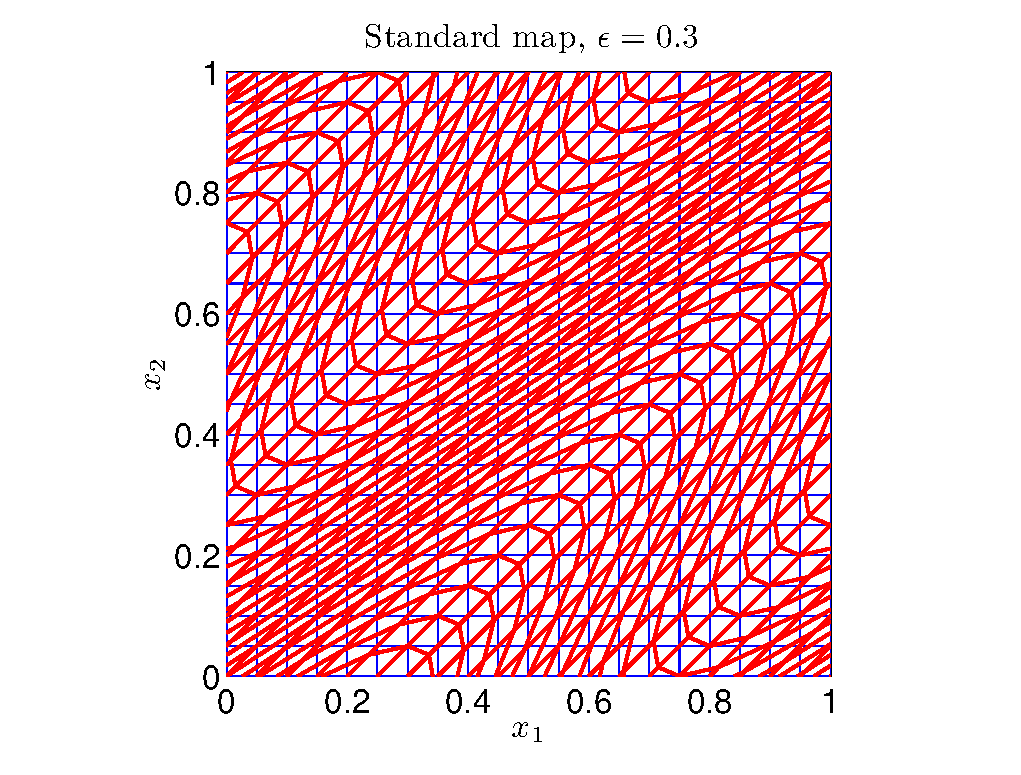
\includegraphics[width=0.45\textwidth,trim=2cm 1cm 2cm 0cm]{standardmapgrid}\\
      \begin{minipage}[s]{0.45\textwidth}
    \begin{eqnarray*}
       \text{Blue grids}:& a_i\\
       \text{Red  grids}:& S^{-1}(a_i)
    \end{eqnarray*}
      \end{minipage}
   \end{tabular}&
  \begin{minipage}[s]{0.45\textwidth}
   \begin{itemize}
    \item $X = [0,1] \times[0,1]$.
    \item $a_i, i=\{1,2,\cdots,n^2\}$ be regualr $n$ by $n$ grids on $X$.
    \item $\bar{\omega}$ is the invariant measure of $S$.
   \end{itemize}
   The optimal model of Perron-Frobenius operator $A_n$ has 
   \begin{eqnarray}
     \label{Anij}
     (A_n)_{ij} =  \frac{\bar{\omega}(S^{-1}(a_j)\cap a_i)}{\bar{\omega}(a_j)}  \nonumber
    \end{eqnarray} 
   \end{minipage}
\end{tabular}

\end{frame}


%%%%%%%%%%%%%%%%%%%%%%%%%%%%%%%%%%%%%%%%%%%%%%%%%%%%%%%%%%%%%%%%%%%%%%%%%
%%%%%%%%%%%%%%%%%%%%%%%%%%%%%%%%%%%%%%%%%%%%%%%%%%%%%%%%%%%%%%%%%%%%%%%%%
\begin{frame}
\myframetitle{Standard Map Simulation}
%%%%%%%%%%%%%%%%%%%%%%%%%%%%%%%%%%%%%%%%%%%%%%%%%%%%%%%%%%%%%%%%%%%%%%%%%
\begin{center}
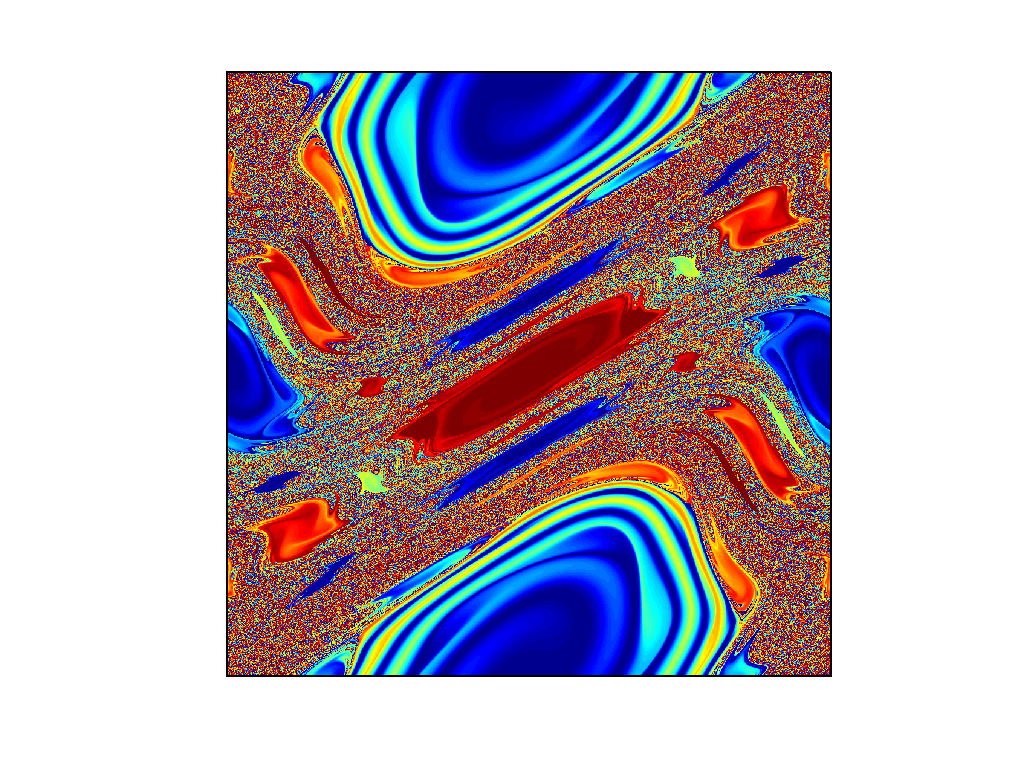
\includegraphics[width=0.45\textwidth,trim=1cm 1cm 0cm 0cm]{standardmapsimuexact}
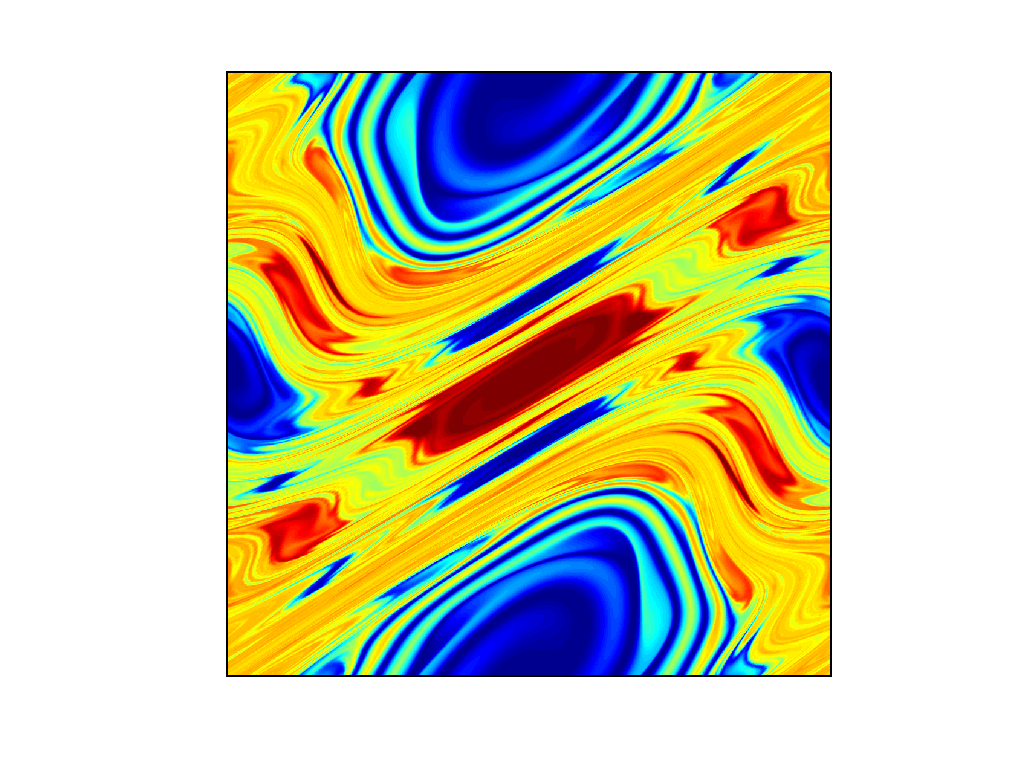
\includegraphics[width=0.45\textwidth,trim=1cm 1cm 0cm 0cm]{standardmapsimumarkov}
\end{center}
\end{frame}




%%%%%%%%%%%%%%%%%%%%%%%%%%%%%%%%%%%%%%%%%%%%%%%%%%%%%%%%%%%%%%%%%%%%%%%%%
%%%%%%%%%%%%%%%%%%%%%%%%%%%%%%%%%%%%%%%%%%%%%%%%%%%%%%%%%%%%%%%%%%%%%%%%%
\begin{frame}
\myframetitle{Standard Map Simulation in Frequency Domain}
%%%%%%%%%%%%%%%%%%%%%%%%%%%%%%%%%%%%%%%%%%%%%%%%%%%%%%%%%%%%%%%%%%%%%%%%%
\begin{center}
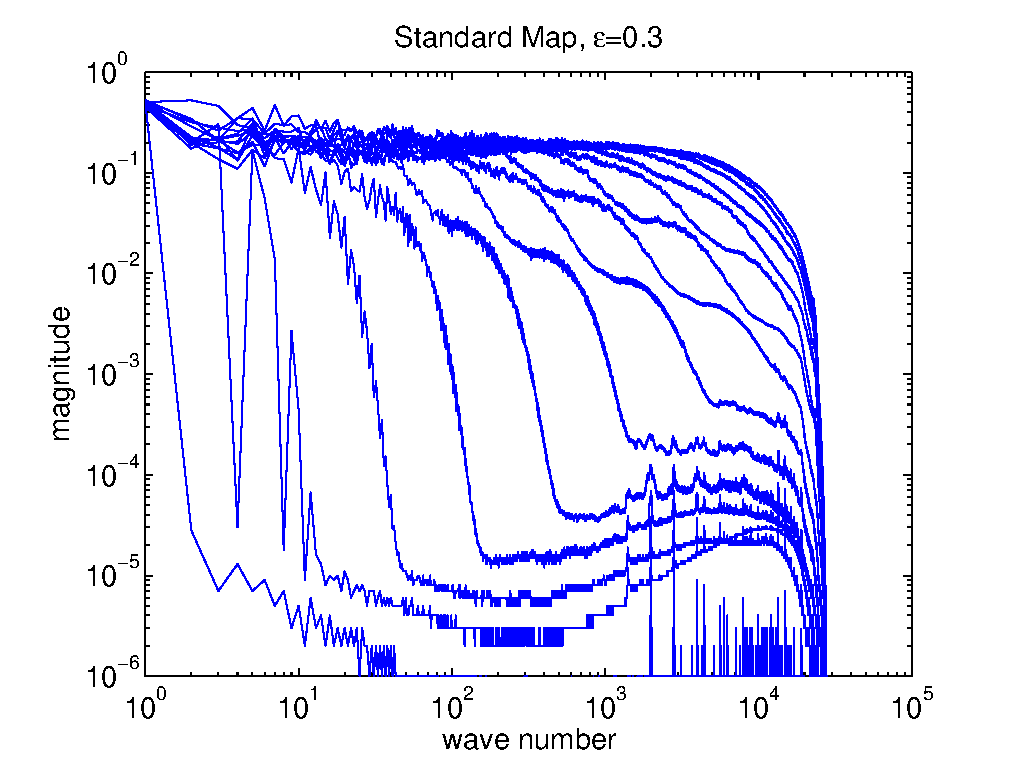
\includegraphics[width=0.45\textwidth,trim=1cm 1cm 0cm 0cm]{standardmapfreqevolve}
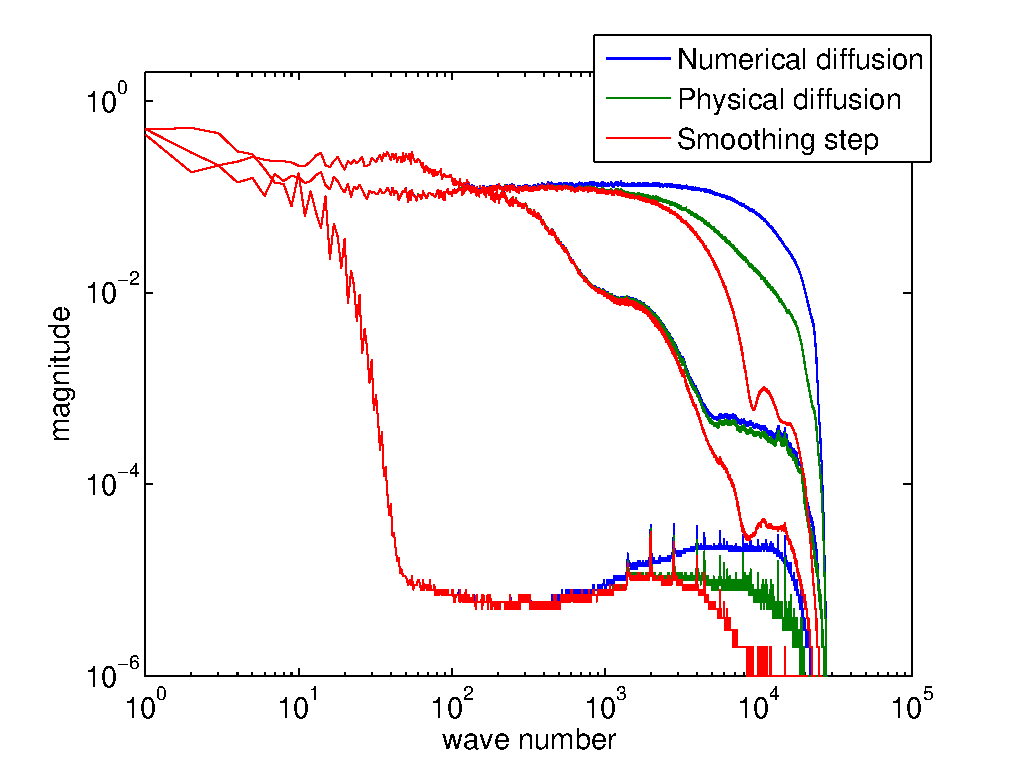
\includegraphics[width=0.45\textwidth,trim=1cm 1cm 0cm 0cm]{standardmapfreqcompare}
\end{center}
\end{frame}


%%%%%%%%%%%%%%%%%%%%%%%%%%%%%%%%%%%%%%%%%%%%%%%%%%%%%%%%%%%%%%%%%%%%%%%%%
%%%%%%%%%%%%%%%%%%%%%%%%%%%%%%%%%%%%%%%%%%%%%%%%%%%%%%%%%%%%%%%%%%%%%%%%%
\begin{frame}
\myframetitle{Evidence of Standard Map Cutoff}
%%%%%%%%%%%%%%%%%%%%%%%%%%%%%%%%%%%%%%%%%%%%%%%%%%%%%%%%%%%%%%%%%%%%%%%%%
\begin{center}
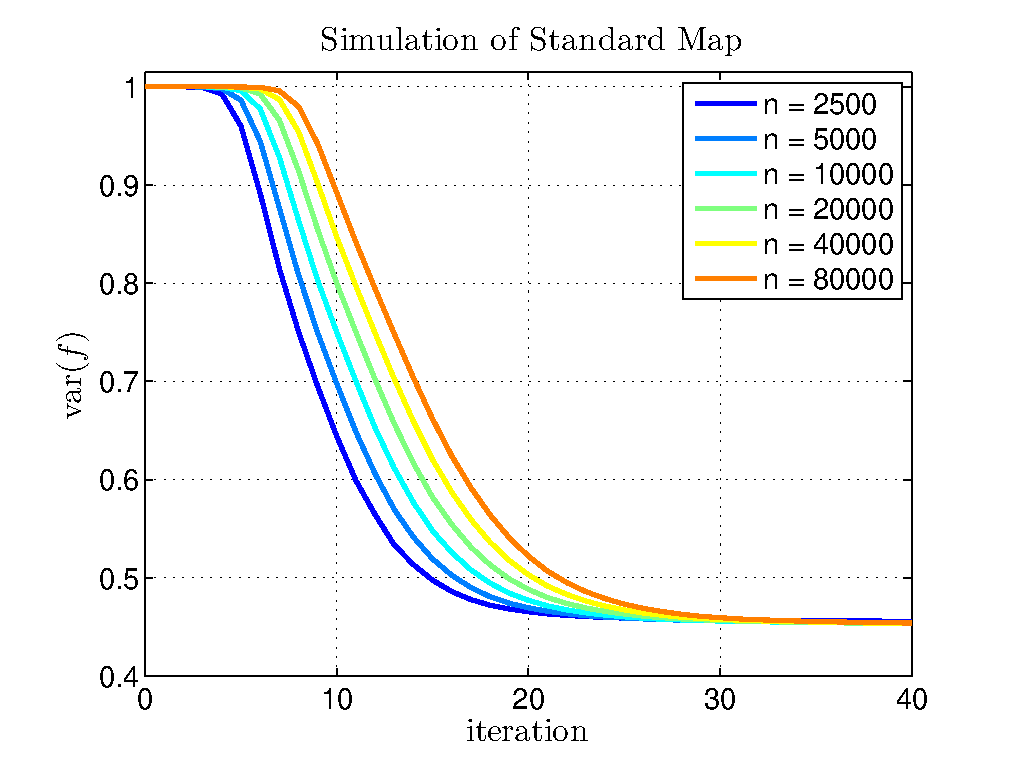
\includegraphics[width=0.45\textwidth,trim=1cm 1cm 0cm 0cm]{standardmapcutoff}
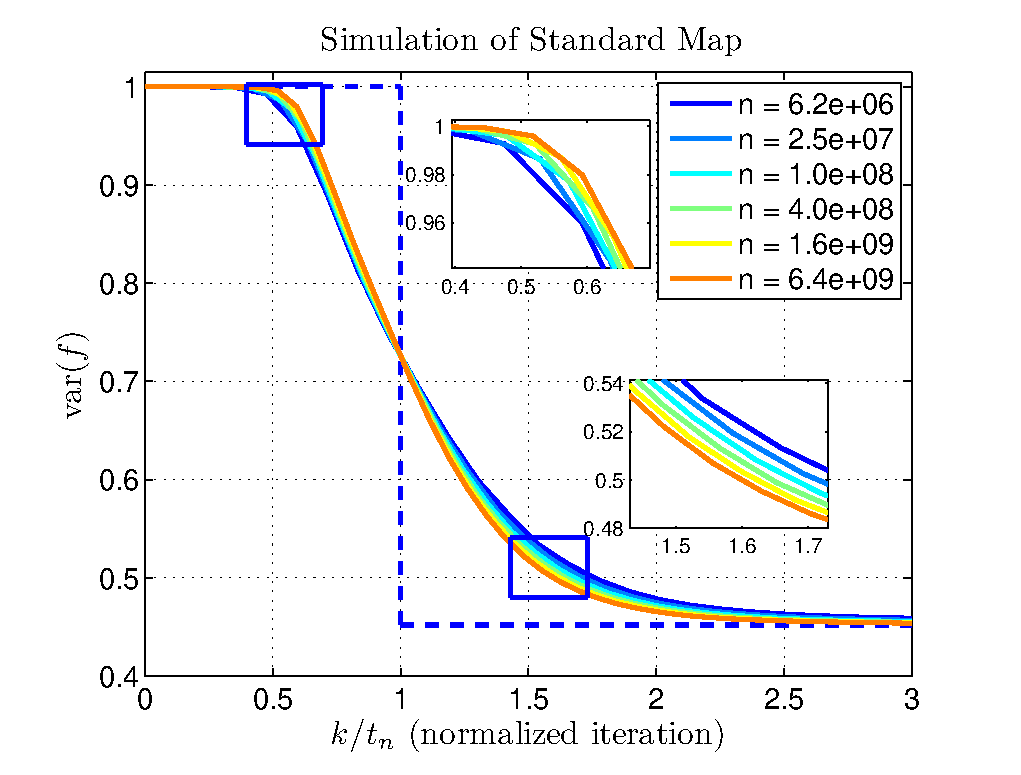
\includegraphics[width=0.45\textwidth,trim=1cm 1cm 0cm 0cm]{standardmapcutoffn}
\end{center}
\begin{itemize}
\item Standard map, $\epsilon = 0.3$, $f^0 = \cos(2\pi x_2)$.
\item $(M,m) = (1,0.4521)$, Cutoff time: $t_n =\min \{ k \mid \text{var}(f^k_n)< \frac{M+m}{2}\} $
\end{itemize}
\end{frame}
%%%%%%%%%%%%%%%%%%%%%%%%%%%%%%%%%%%%%%%%%%%%%%%%%%%%%%%%%%%%%%%%%%%%%%%%%
%%%%%%%%%%%%%%%%%%%%%%%%%%%%%%%%%%%%%%%%%%%%%%%%%%%%%%%%%%%%%%%%%%%%%%%%%
\begin{frame}
\myframetitle{Evidence of Standard Map Cutoff}
%%%%%%%%%%%%%%%%%%%%%%%%%%%%%%%%%%%%%%%%%%%%%%%%%%%%%%%%%%%%%%%%%%%%%%%%%
\begin{center}
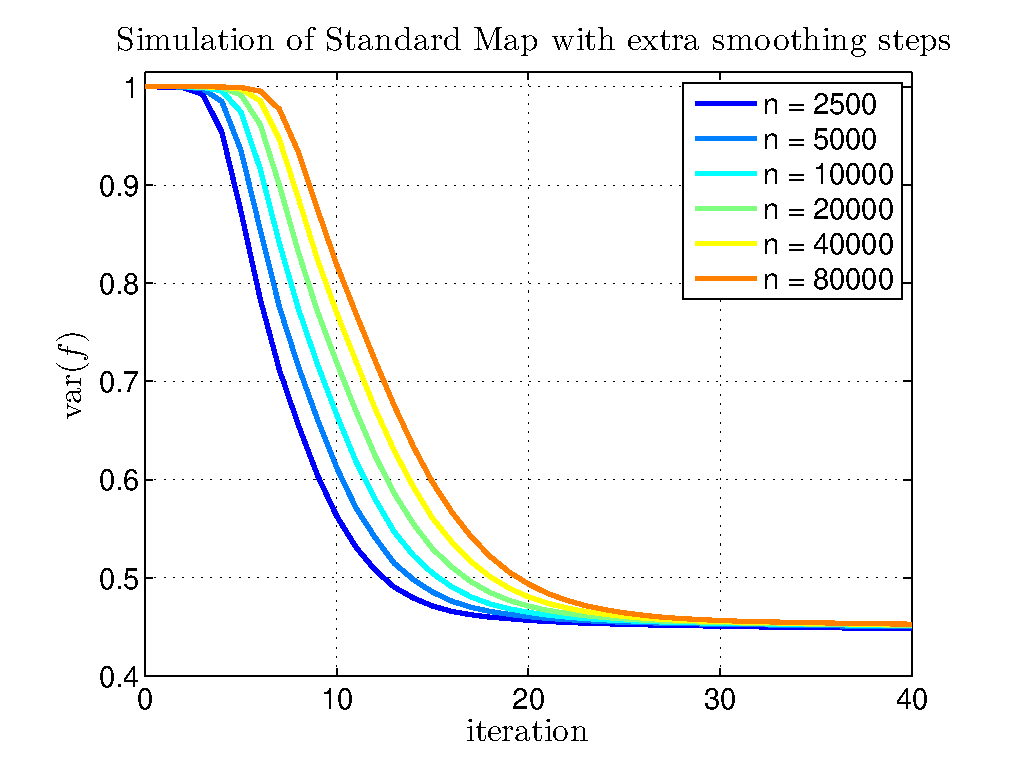
\includegraphics[width=0.45\textwidth,trim=1cm 1cm 0cm 0cm]{standardmapcutoffwithsmoothing}
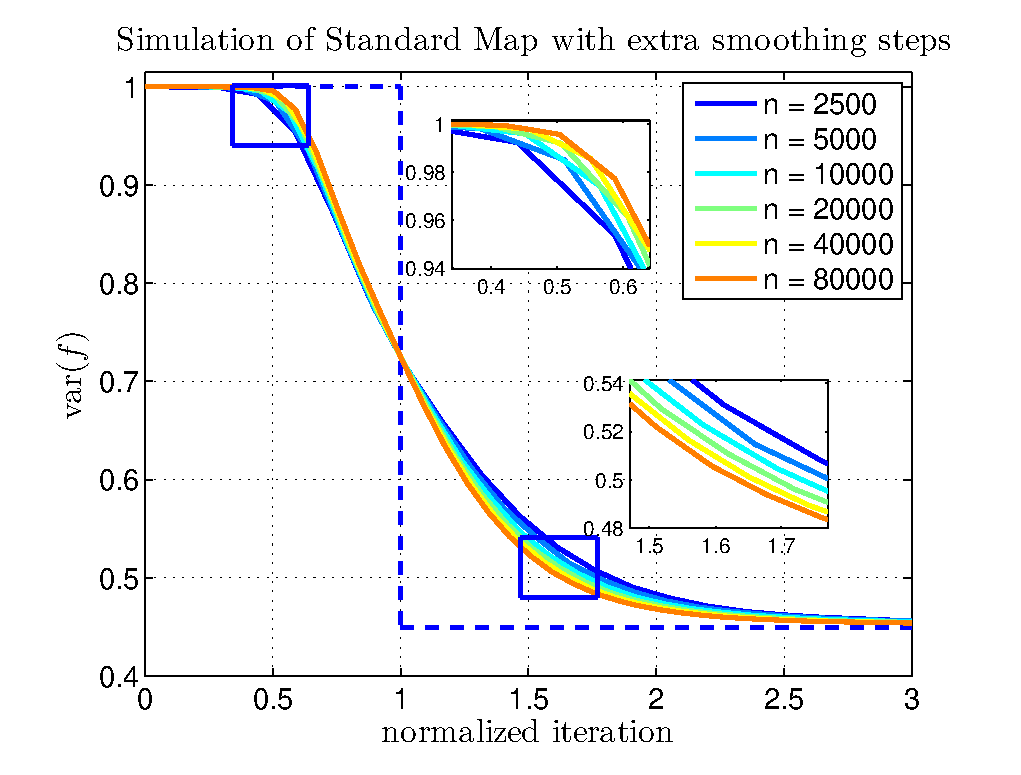
\includegraphics[width=0.45\textwidth,trim=1cm 1cm 0cm 0cm]{standardmapcutoffwithsmoothingn}
\end{center}

\begin{itemize}
\item Standard map, $\epsilon = 0.3$, $f^0 = \cos(2\pi x_2)$, with additional smoothing steps after each iteration.
\item $(M,m) = (1,0.4498)$, Cutoff time: $t_n =\min \{ k \mid \text{var}(f^k_n)< \frac{M+m}{2}\} $
\end{itemize}

\end{frame}


%%%%%%%%%%%%%%%%%%%%%%%%%%%%%%%%%%%%%%%%%%%%%%%%%%%%%%%%%%%%%%%%%%%%%%%%%
\begin{frame}
\myframetitle{Glesson's Simulation}
%%%%%%%%%%%%%%%%%%%%%%%%%%%%%%%%%%%%%%%%%%%%%%%%%%%%%%%%%%%%%%%%%%%%%%%%%
\begin{center}
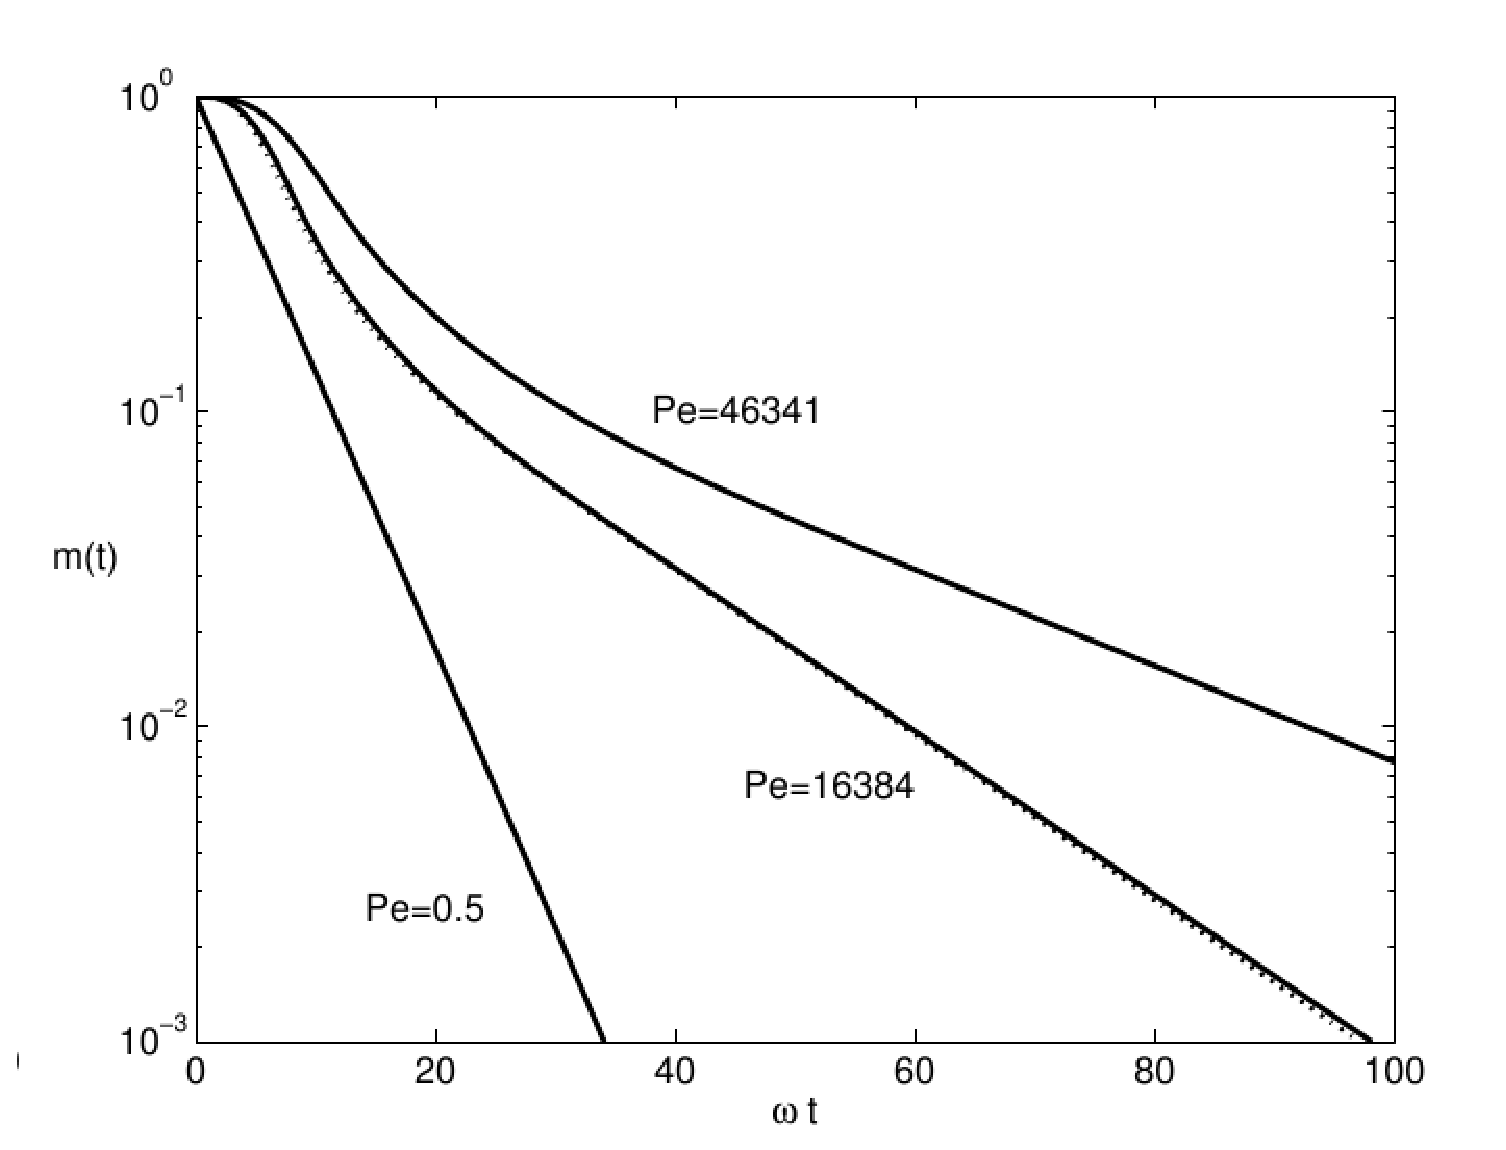
\includegraphics[width=0.65\textwidth]{Glessonstandardmap}
\end{center}
\end{frame}

%%%%%%%%%%%%%%%%%%%%%%%%%%%%%%%%%%%%%%%%%%%%%%%%%%%%%%%%%%%%%%%%%%%%%%%%%
%%%%%%%%%%%%%%%%%%%%%%%%%%%%%%%%%%%%%%%%%%%%%%%%%%%%%%%%%%%%%%%%%%%%%%%%%
%%%%%%%%%%%%%%%%%%%%%%%%%%%%%%%%%%%%%%%%%%%%%%%%%%%%%%%%%%%%%%%%%%%%%%%%%
\begin{frame}
\myframetitle{Modified Cat map Simulation}
%%%%%%%%%%%%%%%%%%%%%%%%%%%%%%%%%%%%%%%%%%%%%%%%%%%%%%%%%%%%%%%%%%%%%%%%%
\begin{center}
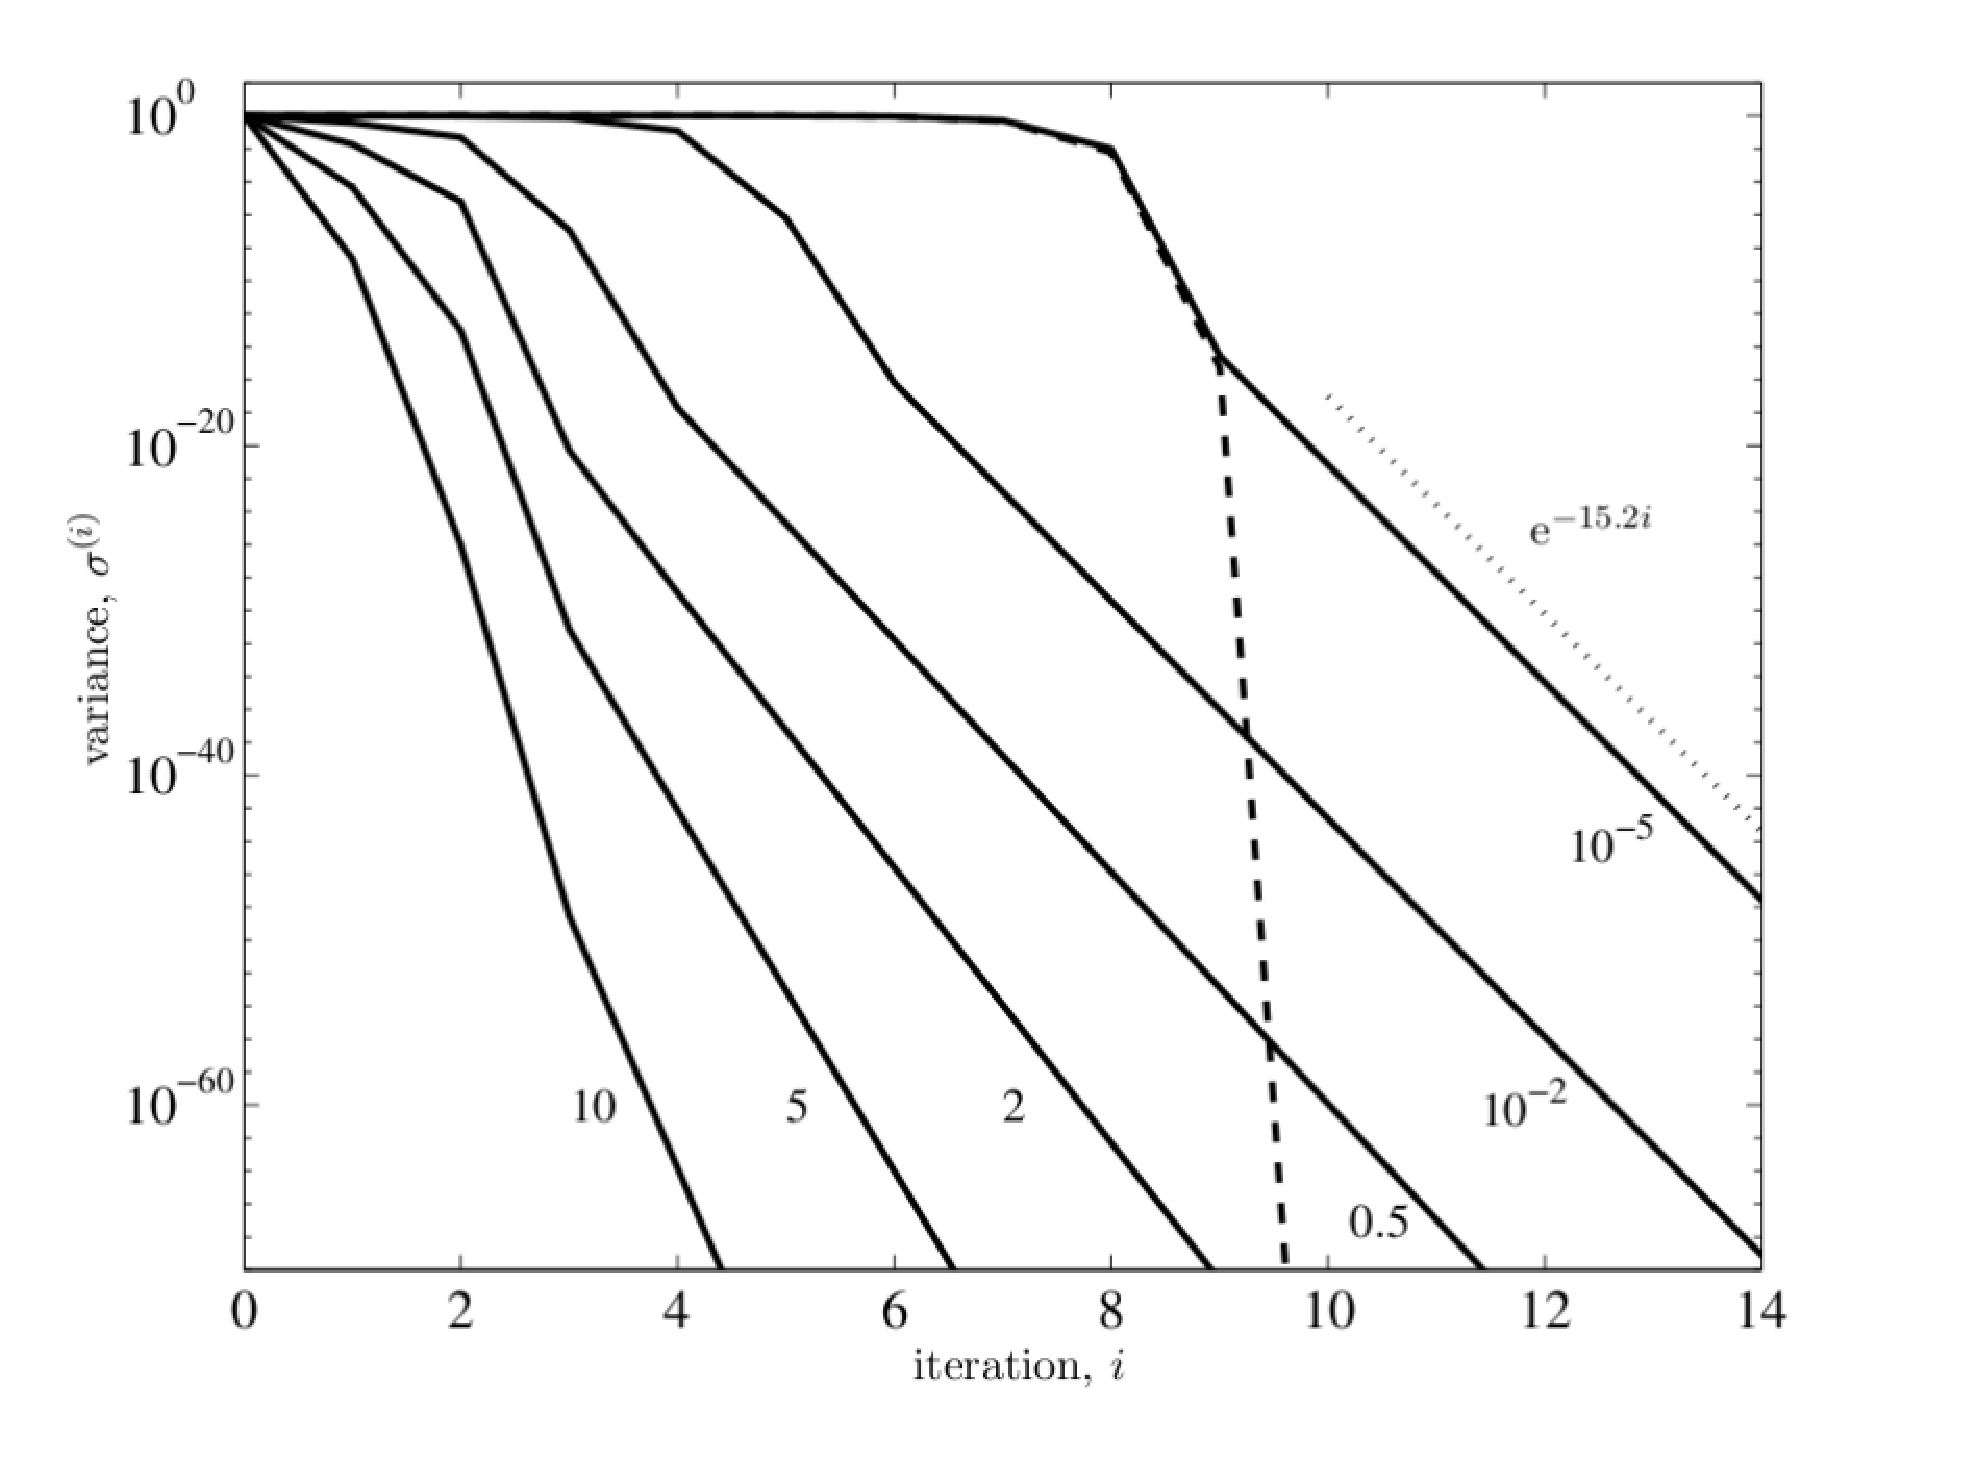
\includegraphics[width=0.65\textwidth]{catmap}
\end{center}
\end{frame}
%%%%%%%%%%%%%%%%%%%%%%%%%%%%%%%%%%%%%%%%%%%%%%%%%%%%%%%%%%%%%%%%%%%%%%%%%
%%%%%%%%%%%%%%%%%%%%%%%%%%%%%%%%%%%%%%%%%%%%%%%%%%%%%%%%%%%%%%%%%%%%%%%%%
%%%%%%%%%%%%%%%%%%%%%%%%%%%%%%%%%%%%%%%%%%%%%%%%%%%%%%%%%%%%%%%%%%%%%%%%%
%%%%%%%%%%%%%%%%%%%%%%%%%%%%%%%%%%%%%%%%%%%%%%%%%%%%%%%%%%%%%%%%%%%%%%%%%
\begin{frame}
\myframetitle{Evidence of Standard Map Cutoff}
%%%%%%%%%%%%%%%%%%%%%%%%%%%%%%%%%%%%%%%%%%%%%%%%%%%%%%%%%%%%%%%%%%%%%%%%%
\begin{center}
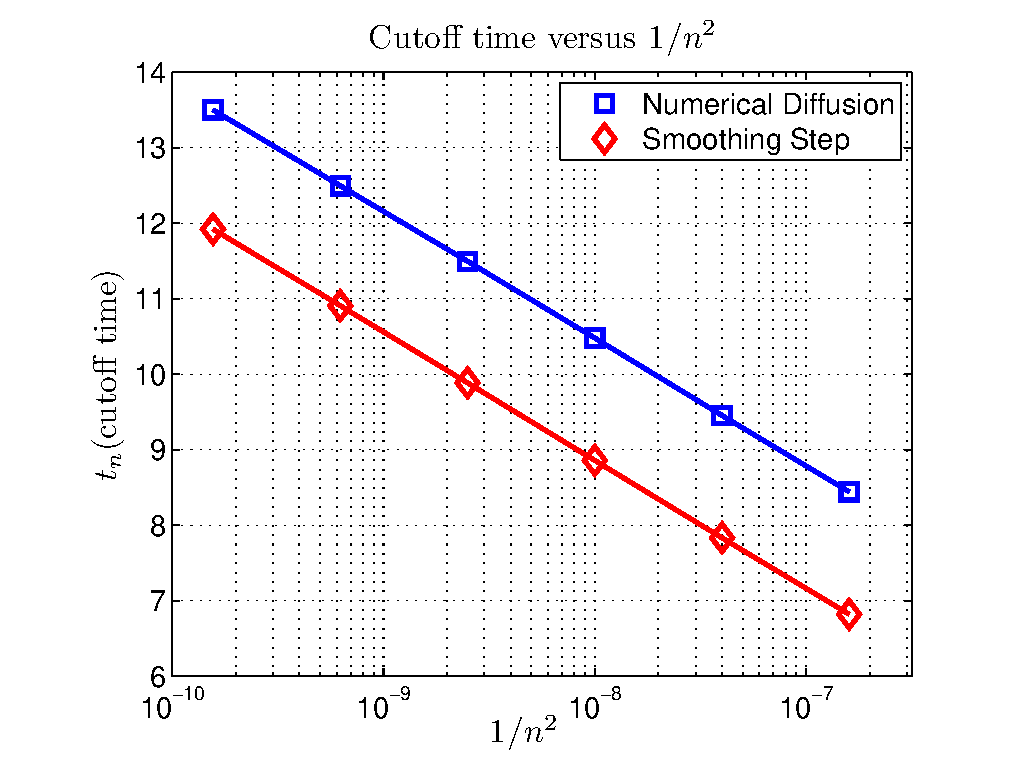
\includegraphics[width=0.45\textwidth,trim=1cm 1cm 0cm 0cm]{cutofftimevsD}
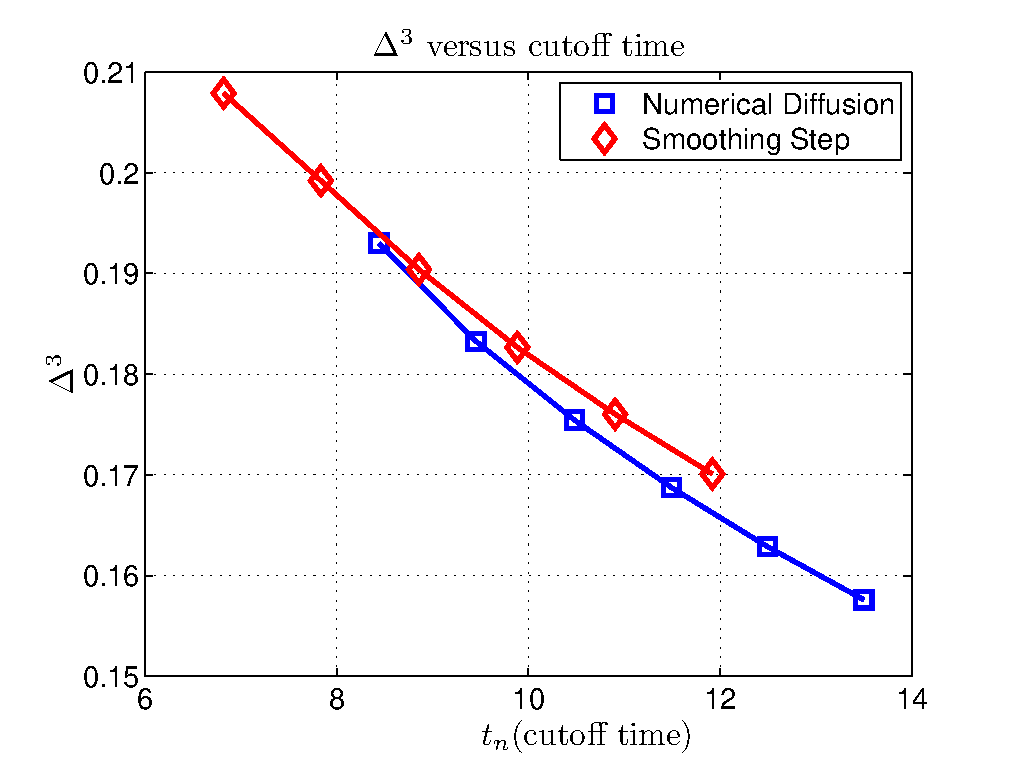
\includegraphics[width=0.45\textwidth,trim=1cm 1cm 0cm 0cm]{areavscutofftime}
\end{center}
\begin{itemize}
\item Cutoff time: $t_n =\min \{ k \mid \text{var}(f^k_n)< \frac{M+m}{2}\} $,
\item $\Delta_{\star}^l\equiv \int_0^l | \nu_{{\star}_\infty}(x)-\nu_{{\star}_n}(x)|dx$, $\star=\{A_n,\bar{A}_n\}$
\end{itemize}

\end{frame}

%%%%%%%%%%%%%%%%%%%%%%%%%%%%%%%%%%%%%%%%%%%%%%%%%%%%%%%%%%%%%%%%%%%%%%%%%
%%%%%%%%%%%%%%%%%%%%%%%%%%%%%%%%%%%%%%%%%%%%%%%%%%%%%%%%%%%%%%%%%%%%%%%%%
\begin{frame}
  \myframetitle{What creates the ``normal'' shape?}

  \centerline{
   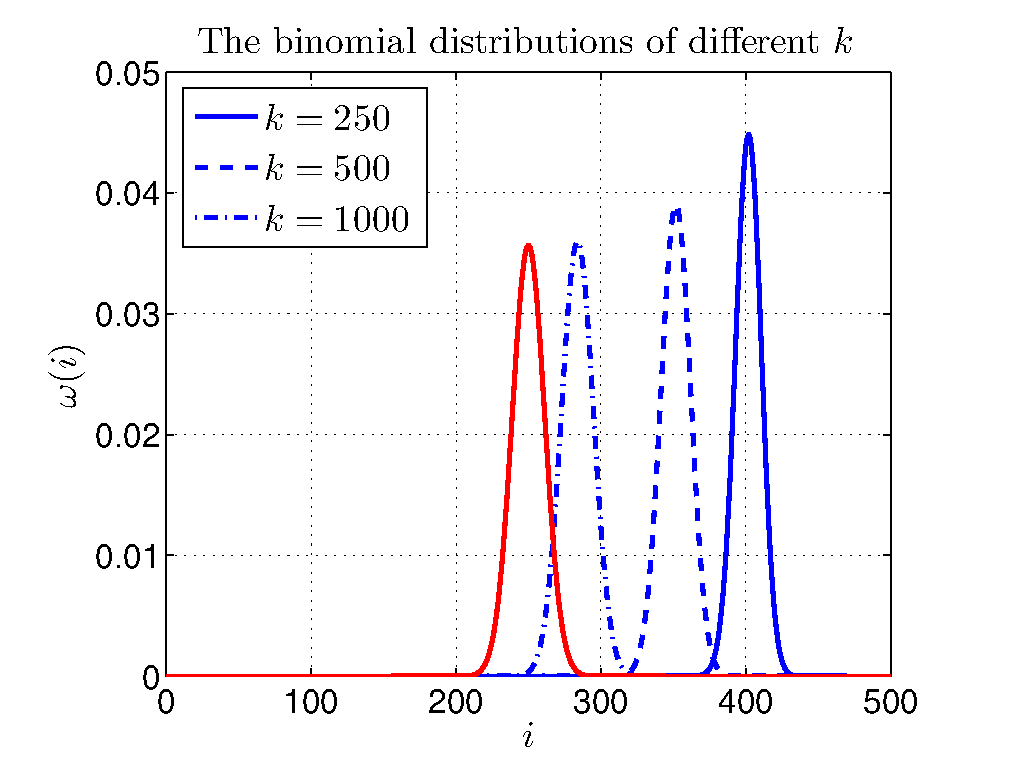
\includegraphics[width=0.45\textwidth]{deltaMexample2a}
         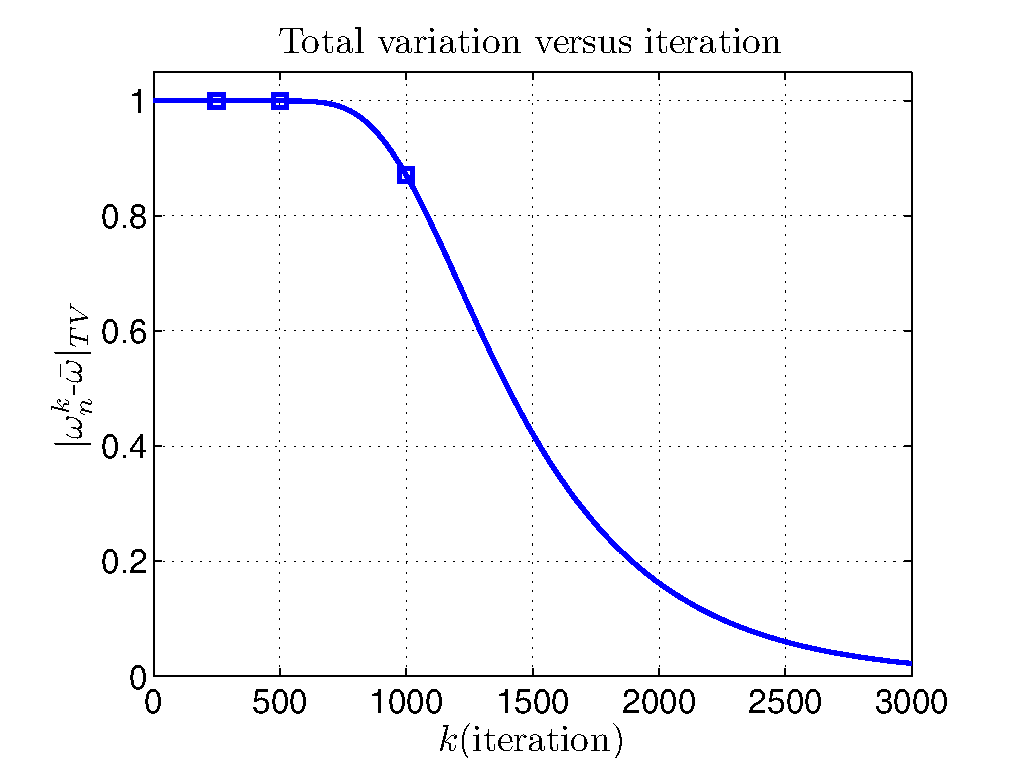
\includegraphics[width=0.45\textwidth]{ehrenfasttv}
  }
  \begin{itemize}
  \item When $n$ is large, binomial distribution converges normal distribution.
  \item The TV between two normal distributions converges to an error function.
  \end{itemize}
\end{frame}




%%%%%%%%%%%%%%%%%%%%%%%%%%%%%%%%%%%%%%%%%%%%%%%%%%%%%%%%%%%%%%%%%%%%%%%%%
%%%%%%%%%%%%%%%%%%%%%%%%%%%%%%%%%%%%%%%%%%%%%%%%%%%%%%%%%%%%%%%%%%%%%%%%%
\begin{frame}
\myframetitle{Symbolic Dynamics(for $1$-D Chaotic Maps) }
%%%%%%%%%%%%%%%%%%%%%%%%%%%%%%%%%%%%%%%%%%%%%%%%%%%%%%%%%%%%%%%%%%%%%%%%%

\begin{itemize}\setlength{\parskip}{0pt}  \setlength{\itemsep}{5pt} \setlength{\topsep}{0pt}
     \item Symbol list $\mathcal{S} = \{L,R\}$. Map $S$ has invariant set $\Lambda$, $x\in \Lambda$
     \item  $s_i \in \mathcal{S}$, $s= \{.s_0s_1\cdots s_n\cdots\} \in \Sigma$
     \item  $\phi: \Lambda \rightarrow \Sigma$
     \item $\sigma: \Sigma \rightarrow \Sigma $, shift operator
           $$\sigma(s)= \{.s_1s_2\cdots s_n\cdots\}$$
     \item $S(x) = \phi^{-1}\circ \sigma \circ \phi(x)$,
           \begin{equation*}
          \xymatrix{
              \Lambda  \ar[d]_{\phi} \ar[r]^{S}
              & \Lambda   \ar[d]^{\phi} \\
          \Sigma \ar[r]_{\sigma}
              & \Sigma}
           \end{equation*}
\end{itemize}

\end{frame}
%%%%%%%%%%%%%%%%%%%%%%%%%%%%%%%%%%%%%%%%%%%%%%%%%%%%%%%%%%%%%%%%%%%%%%%%%
%%%%%%%%%%%%%%%%%%%%%%%%%%%%%%%%%%%%%%%%%%%%%%%%%%%%%%%%%%%%%%%%%%%%%%%%%
\begin{frame}
\myframetitle{Symbolic Dynamics }
%%%%%%%%%%%%%%%%%%%%%%%%%%%%%%%%%%%%%%%%%%%%%%%%%%%%%%%%%%%%%%%%%%%%%%%%%

\centerline{
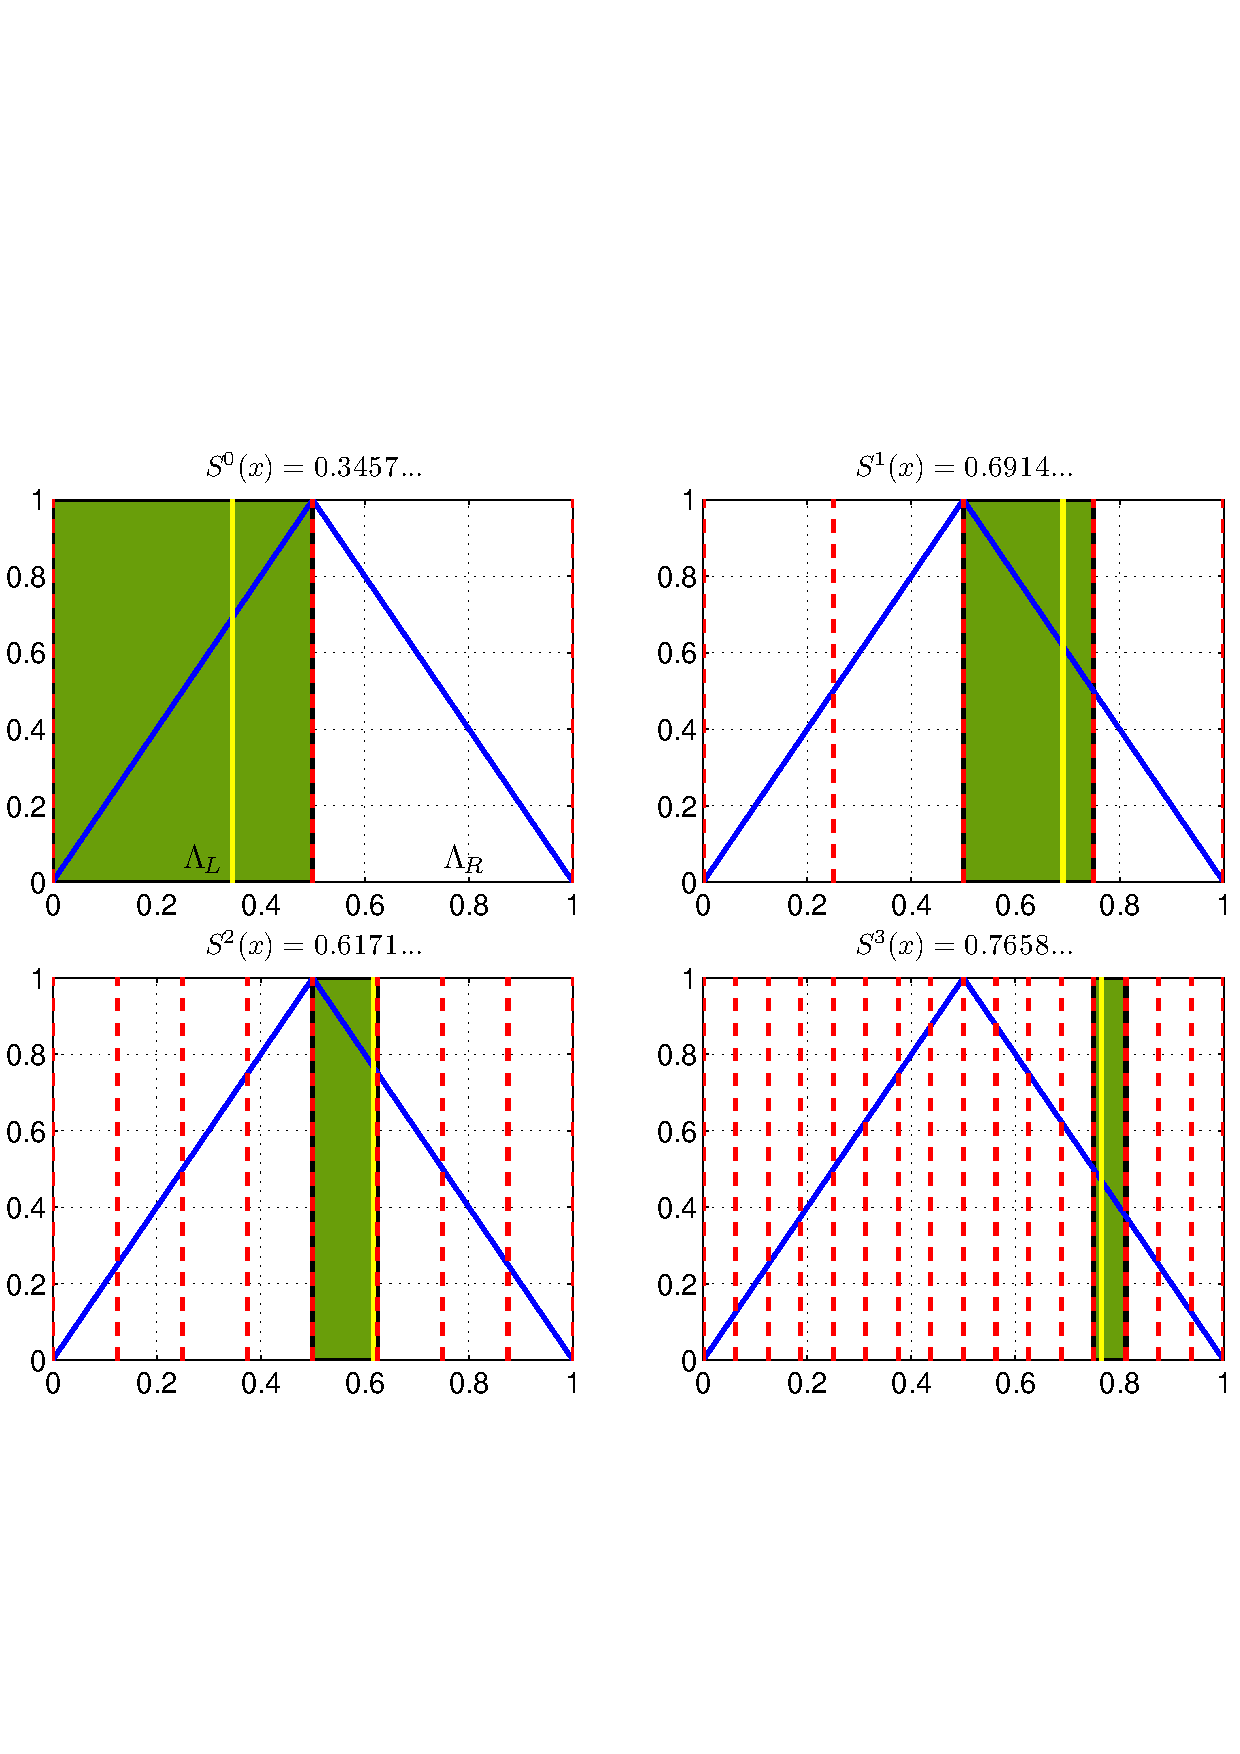
\includegraphics[width=0.7\textwidth]{tentmapplot2}
}
$x = 0.3457...  $, and $ \phi(x)=\{.LRRR...\}$.

\end{frame}
%%%%%%%%%%%%%%%%%%%%%%%%%%%%%%%%%%%%%%%%%%%%%%%%%%%%%%%%%%%%%%%%%%%%%%%%%
%%%%%%%%%%%%%%%%%%%%%%%%%%%%%%%%%%%%%%%%%%%%%%%%%%%%%%%%%%%%%%%%%%%%%%%%%
\begin{frame}
\myframetitle{Stochastic Symbol Sequence }
%%%%%%%%%%%%%%%%%%%%%%%%%%%%%%%%%%%%%%%%%%%%%%%%%%%%%%%%%%%%%%%%%%%%%%%%%
\begin{itemize}\setlength{\parskip}{0pt}  \setlength{\itemsep}{5pt} \setlength{\topsep}{0pt}
    \item Similar to symbolic dynamics, we want to use a sequence of numbers to represent a distribution in
          $\Omega \in L^{\infty}[\Lambda], \int_{\Lambda}dx=1 $.
\end{itemize}

\begin{definition} \textbf{Stochastic symbol sequence.}
Consider $\mathcal{S}$ to be the symbol list. Let $\Delta$ be the collection of all
semi-infinite sequences of elements in $[0,1]$. We define $\delta^\star \in \Delta$ for each
symbol $\star \in \mathcal{S}$ as
 \begin{align}
 \begin{split}
 \delta^\star &= \{.\delta_0^\star \delta_1^\star\cdots \delta_n^\star\cdots\} \\
 %\delta^R &= \{.\delta_0^R \delta_1^R\cdots \delta_n^R\cdots\}
 \end{split}
 \end{align}
with $\delta^\star_i \in [0,1]$ for all $i$.
\end{definition}
\begin{itemize}\setlength{\parskip}{0pt}  \setlength{\itemsep}{5pt} \setlength{\topsep}{0pt}
  \item $\sigma: \Delta \rightarrow \Delta $, shift operator
    $$\sigma(\delta^L)= \{.\delta^L_1\delta^L_2\cdots
           \delta^L_n\cdots\}$$
\end{itemize}

\end{frame}
%%%%%%%%%%%%%%%%%%%%%%%%%%%%%%%%%%%%%%%%%%%%%%%%%%%%%%%%%%%%%%%%%%%%%%%%%
%%%%%%%%%%%%%%%%%%%%%%%%%%%%%%%%%%%%%%%%%%%%%%%%%%%%%%%%%%%%%%%%%%%%%%%%%
\begin{frame}
\myframetitle{Stochastic Symbol Sequence }
%%%%%%%%%%%%%%%%%%%%%%%%%%%%%%%%%%%%%%%%%%%%%%%%%%%%%%%%%%%%%%%%%%%%%%%%%

\begin{itemize}\setlength{\parskip}{0pt}  \setlength{\itemsep}{5pt} \setlength{\topsep}{0pt}

    \item Consider $\mathcal{S} =\{L,R \}$, $\psi^L :\Omega \rightarrow \Delta$
               \begin{eqnarray}
               \label{psidef}
               %\delta^L_i = \int_{\Lambda_L} P^i_S \omega(x)dx \text{,   and  }
               \delta^L_i = \int_{\Lambda_L} P^i_S \left(\omega(x)\right)dx \text{, for all }i\ge0
               \end{eqnarray}
    \item For $x\in \Lambda$ having distribution $\omega$, the interpretation of $\delta_i^L$ is
             \begin{eqnarray}
             \label{deltaistar}
             \delta_i^L = \prob(\phi(x)_i = L) \text{, for } \text{ for all }i
              \end{eqnarray}


    \item If there are only two symbols $\mathcal{S} =\{L,R\}$, $\delta^R=1-\delta^L$.
    \item  Define $\psi \equiv \psi^L$, we have,
           \begin{lemma}
                $$\psi \circ P_S = \sigma \circ \psi$$
           \end{lemma}

\end{itemize}

   %\item  $\mathcal{S} = \{L,R\}$, $\delta_i^{L},\delta_i^{R} \in [0, 1]$,
   %        \begin{eqnarray}
   %        \delta^L = \{\cdots \delta_{-n}^L\cdots \delta_{-1}^L.\delta_0^L \delta_1^L\cdots \delta_n^L\cdots\} \nonumber\\
   %        \delta^R = \{\cdots \delta_{-n}^R\cdots \delta_{-1}^R.\delta_0^R \delta_1^R\cdots \delta_n^R\cdots\} \nonumber
   %        \end{eqnarray}

    %
    %$$\sigma(\delta^L)= \{\cdots \delta^L_{-n}\cdots \delta^L_{-1}\delta^L_0.\delta^L_1\cdots
    %       \delta^L_n\cdots\}$$

\end{frame}

%%%%%%%%%%%%%%%%%%%%%%%%%%%%%%%%%%%%%%%%%%%%%%%%%%%%%%%%%%%%%%%%%%%%%%%%%
%%%%%%%%%%%%%%%%%%%%%%%%%%%%%%%%%%%%%%%%%%%%%%%%%%%%%%%%%%%%%%%%%%%%%%%%%
\begin{frame}
\myframetitle{Stochastic Symbol Sequence }
%%%%%%%%%%%%%%%%%%%%%%%%%%%%%%%%%%%%%%%%%%%%%%%%%%%%%%%%%%%%%%%%%%%%%%%%%

\begin{itemize}\setlength{\parskip}{0pt}  \setlength{\itemsep}{5pt} \setlength{\topsep}{0pt}
   \item Unfortunately, $\psi$ is not invertible. There are many $\omega\in \Omega$ which maps to the same $\delta$
   \item So we restrict $\omega$ to the following space,
        \begin{eqnarray}
        \label{DefOmegabar}
        \bar{\Omega} = \left\{ \omega \left| \omega(x) = \lim_{n \rightarrow \infty} \prod_{i=0}^n \beta^{\phi(x)_i}_i \right. \right\}
        \end{eqnarray}
        where $\beta^L_i \in [0,1]$, $\beta^R_i=1-\beta^L_i$.
         Then $\psi:\bar{\Omega} \rightarrow \Delta$ is invertible.

    \item For $\omega \in \bar{\Omega}$, $\delta^L_i=\psi(\omega)_i = \beta^L_i$ for all $i$
    \item For $x \in \Lambda$ having pdf $\omega\in \bar{\Omega}$, and any $s^*\in \Sigma$, one has
         \begin{eqnarray*}
             \prob(\phi(x)_i=s_i^*) = 
             \prob(\phi(x)_i=s_i^* \mid  \phi(x)_k=s_k^*, \text{ for all } k \neq i )
          \end{eqnarray*}


\end{itemize}

This lemma says given $s_k$ does not help to know $s_i$. 


\end{frame}
%%%%%%%%%%%%%%%%%%%%%%%%%%%%%%%%%%%%%%%%%%%%%%%%%%%%%%%%%%%%%%%%%%%%%%%%%
%%%%%%%%%%%%%%%%%%%%%%%%%%%%%%%%%%%%%%%%%%%%%%%%%%%%%%%%%%%%%%%%%%%%%%%%%
\begin{frame}
\myframetitle{Stochastic Symbol Sequence }
%%%%%%%%%%%%%%%%%%%%%%%%%%%%%%%%%%%%%%%%%%%%%%%%%%%%%%%%%%%%%%%%%%%%%%%%%
\begin{itemize}\setlength{\parskip}{0pt}  \setlength{\itemsep}{5pt} \setlength{\topsep}{0pt}

   \item $P_S$ is the Perron-Frobenius operator of $S$
         \begin{eqnarray}
         P_S (\omega) \in \bar{\Omega}, \mbox{if } \omega \in \bar{\Omega} \nonumber
         \end{eqnarray}
   \item More importantly,
         \begin{eqnarray}
         P_S= \psi^{-1}\circ \sigma \circ \psi  \nonumber
         \end{eqnarray}
   \item Reminder: the above procedure is to find the subspace $\bar{\Omega}$ such that when $\omega\in\bar{\Omega}$, we can find $P_S^i(\omega)$ for all $i$ easily.
\end{itemize}

\end{frame}
%%%%%%%%%%%%%%%%%%%%%%%%%%%%%%%%%%%%%%%%%%%%%%%%%%%%%%%%%%%%%%%%%%%%%%%%%
%%%%%%%%%%%%%%%%%%%%%%%%%%%%%%%%%%%%%%%%%%%%%%%%%%%%%%%%%%%%%%%%%%%%%%%%%
\begin{frame}
\myframetitle{Total Variation Distance in $\bar{\Omega}$}
%%%%%%%%%%%%%%%%%%%%%%%%%%%%%%%%%%%%%%%%%%%%%%%%%%%%%%%%%%%%%%%%%%%%%%%%%
\begin{itemize}\setlength{\parskip}{0pt}  \setlength{\itemsep}{5pt} \setlength{\topsep}{0pt}
    \item $\omega$, $\hat{\omega}\in{\bar{\Omega}}$ have stochastic symbol sequences  $\{\delta^L, \delta^R\}$ and $\{\hat{\delta}^L,\hat{\delta}^R \}$, respectively.
          \begin{eqnarray}
            \label{infiniteTV}
            |\omega-\hat{\omega}|_{TV} = \frac{1}{2} \lim_{n \rightarrow \infty}  \sum_{s\in\Sigma} \left|
                                     \prod_{i=0}^n\delta_i^{s_i}-\prod_{i=0}^n\hat{\delta}_i^{s_i}  \right| \nonumber
          \end{eqnarray}
    \item $\delta_i^L = \hat{\delta}_i^L$ when $i\notin \theta$, and $|\theta| = p$.
          \begin{eqnarray}
           \label{finiteTV}
            |\omega-\hat{\omega}|_{TV} = \frac{1}{2} \sum_{s\in\Sigma_p}  \left|
                             \prod_{i\in \theta}\delta_i^{s_i}-\prod_{i\in\theta}\hat{\delta}_i^{s_i}  \right| \nonumber
          \end{eqnarray}
   where $\Sigma_p$ are all combinations of $p$ symbols($2^p$).
   %\item without loss of generality, assume $\delta^L_i =\delta^R_i$ for all $i$, and let $\delta \equiv \delta^L $
\end{itemize}

\end{frame}

%%%%%%%%%%%%%%%%%%%%%%%%%%%%%%%%%%%%%%%%%%%%%%%%%%%%%%%%%%%%%%%%%%%%%%%%%
%%%%%%%%%%%%%%%%%%%%%%%%%%%%%%%%%%%%%%%%%%%%%%%%%%%%%%%%%%%%%%%%%%%%%%%%%
\begin{frame}
\myframetitle{Total Variation Distance to Invariant Distribution}
%%%%%%%%%%%%%%%%%%%%%%%%%%%%%%%%%%%%%%%%%%%%%%%%%%%%%%%%%%%%%%%%%%%%%%%%%
\begin{itemize}\setlength{\parskip}{0pt}  \setlength{\itemsep}{5pt} \setlength{\topsep}{0pt}
    \item The invariant distribution of map $S$ is $\bar{\omega}$.
          $$\bar{\delta}\equiv \psi(\bar{\omega}) = \left\{.\frac{1}{2}\frac{1}{2}\frac{1}{2}...\right\}  $$
    \item $\omega \mapsto |\omega-\bar{\omega}|_{TV}$ is convex, so  $\delta \mapsto |\psi^{-1}(\delta)-\bar{\omega}|_{TV} $ is also convex.
    \item Using convexity, we can prove
          \begin{lemma}
          \label{alldifflemma}
           $\delta$ and $\hat{\delta}$ are two stochastic symbol sequences, each corresponds to the probability distribution $\omega$ and $\hat{\omega}$, respectively. Suppose there exists a bijection $\beta: i \mapsto j$ such that $|\delta_i-\frac{1}{2}| \ge |\hat{\delta}_j-\frac{1}{2} |$ for all $i\in \mathbb{Z}$, then
          \begin{eqnarray}
          |\omega-\bar{\omega} |_{TV} \ge|\hat{\omega}-\bar{\omega} |_{TV}
          \end{eqnarray}
\end{lemma}
\end{itemize}

\end{frame}
%%%%%%%%%%%%%%%%%%%%%%%%%%%%%%%%%%%%%%%%%%%%%%%%%%%%%%%%%%%%%%%%%%%%%%%%%
%%%%%%%%%%%%%%%%%%%%%%%%%%%%%%%%%%%%%%%%%%%%%%%%%%%%%%%%%%%%%%%%%%%%%%%%%
\begin{frame}
\myframetitle{Evaluate the Total Variation Distance}
%%%%%%%%%%%%%%%%%%%%%%%%%%%%%%%%%%%%%%%%%%%%%%%%%%%%%%%%%%%%%%%%%%%%%%%%%
\begin{itemize}
    \item Consider the flolowing two sequences
        \begin{eqnarray} 
         \hat{\delta} 
               = \{.\underbrace{\hat{\delta}_{\star} \hat{\delta}_{\star} \cdots \hat{\delta}_{\star}}_{p}\frac{1}{2}\frac{1}{2}\cdots\},  
         \bar{\delta}= \left\{.\frac{1}{2}\frac{1}{2}\frac{1}{2}\cdots\right\}\nonumber
        \end{eqnarray}         
        %   $\hat{\delta}_0 =\hat{\delta}_1= \cdots = \hat{\delta}_{p-1}$
   \item The TV can be evaluated by finding the difference between two binomial distributions. %$|\psi^{-1}(\delta)-\psi^{-1}(\bar{\delta)}|^{TV}$
        \begin{eqnarray}
           |\hat{\omega}-\bar{\omega}|_{TV}
                     & = &\frac{1}{2} \sum_{s\in\Sigma_p}
                           \left| \prod_{i\in \theta}\hat{\delta}_i^{s_i}-\prod_{i\in\theta}\bar{\delta}_i^{s_i}  \right| \nonumber \\
                     & = &\frac{1}{2}  \sum_{k=0}^p {p \choose k}
                           \left|(\hat{\delta}_\star)^k (1-\hat{\delta}_\star)^{p-k} - \frac{1}{2^p} \right| \nonumber\\
                     & = &\frac{1}{2} \sum_{k=0}^p\left|\text{binomial}(k;p,\hat{\delta}_\star)-\text{binomial}\left(k;p,\frac{1}{2}\right)\right| \nonumber
     %                & \rightarrow &\erf \left( \sqrt{\frac{p}{2}}\left((\delta_{\star}^m)-\frac{1}{2}\right)\right) \text{, when } p\rightarrow \infty \text{, and } \delta_{\star}^m \rightarrow \frac{1}{2}
                    % & = &\frac{1}{2}  \sum_{k=0}^p \left|{p \choose k}
                    %       (\delta_\star)^k (1-\delta_\star)^{p-k} -{p \choose k} \frac{1}{2^p} \right|\nonumber
        \end{eqnarray}
\end{itemize}


\end{frame}
%%%%%%%%%%%%%%%%%%%%%%%%%%%%%%%%%%%%%%%%%%%%%%%%%%%%%%%%%%%%%%%%%%%%%%%%%
%%%%%%%%%%%%%%%%%%%%%%%%%%%%%%%%%%%%%%%%%%%%%%%%%%%%%%%%%%%%%%%%%%%%%%%%%
\begin{frame}
\myframetitle{Upper Bound and Lower Bound}
%%%%%%%%%%%%%%%%%%%%%%%%%%%%%%%%%%%%%%%%%%%%%%%%%%%%%%%%%%%%%%%%%%%%%%%%%
% the plot of ub,lb theorems
\begin{theorem}\textbf{Lower Bound.}
\label{theoremlb}
$\delta$ and $\bar{\delta}$ are two stochastic symbol sequences, each corresponds to the probability distribution $\omega$ and the invariant distribution $\bar{\omega}$, respectively. Suppose there is a set $\theta \subset \mathbb{Z}^++\{0\} $, $|\theta|=p$ such that for all $i \in \theta$, $|\delta_i-\frac{1}{2}|>\epsilon$, then
\begin{eqnarray}
\label{lbineq}
|\omega-\bar{\omega}|_{TV} \ge \mathbf{I}_{\frac{1}{2}}(p-k^*,k^*+1) - \mathbf{I}_{\frac{1}{2}-\epsilon}(p-k^*,k^*+1)
\end{eqnarray}
with
\begin{eqnarray}
\label{kstar}
k^* =  \left\lfloor p \frac{\log{2}+\log{(\frac{1}{2}-\epsilon)} }{\log{(\frac{1}{2}-\epsilon)}-\log{(\frac{1}{2}+\epsilon})} \right\rfloor
\end{eqnarray}
where $\mathbf{I}$ is the regularized incomplete beta function.
\end{theorem}
In this theorem, we bound $|\omega-\bar{\omega}|_{TV}$ by choosing $\hat{\delta}_\star = \frac{1}{2}+\epsilon$. 

\end{frame}

%%%%%%%%%%%%%%%%%%%%%%%%%%%%%%%%%%%%%%%%%%%%%%%%%%%%%%%%%%%%%%%%%%%%%%%%%
%%%%%%%%%%%%%%%%%%%%%%%%%%%%%%%%%%%%%%%%%%%%%%%%%%%%%%%%%%%%%%%%%%%%%%%%%
\begin{frame}
\myframetitle{The Limit of the Bounds}
%%%%%%%%%%%%%%%%%%%%%%%%%%%%%%%%%%%%%%%%%%%%%%%%%%%%%%%%%%%%%%%%%%%%%%%%%
%\begin{itemize}
%   \item
         \begin{align*}
         \hat{\delta}      = \{.\underbrace{\hat{\delta}_\star \hat{\delta}_\star \cdots \hat{\delta}_\star}_{p}\frac{1}{2}\frac{1}{2}\cdots\}, \,\,\,
         \bar{\delta}  = \left\{.\frac{1}{2}\frac{1}{2}\frac{1}{2}\cdots\right\}
         \end{align*}
%\end{itemize}
\begin{theorem}
\label{theoremapproxlb} $\bar{\omega}$ and $\hat{\omega}$ are two probability distributions, and have the stochastic
symbol sequences $\bar{\delta}$ and $\delta$ as defined above, respectively. Let $p
\rightarrow \infty$ and $\hat{\delta}_{\star} \rightarrow \frac{1}{2}$, then one has
\begin{align}
\begin{split}
  \label{lbublimit}
                 |\hat{\omega}-\bar{\omega}|_{TV}
               & =  \erf \left( \sqrt{\frac{p}{2}}\left((\hat{\delta}_{\star})-\frac{1}{2}\right)\right)
\end{split}
\end{align}


\end{theorem}

\end{frame}

%%%%%%%%%%%%%%%%%%%%%%%%%%%%%%%%%%%%%%%%%%%%%%%%%%%%%%%%%%%%%%%%%%%%%%%%%
%%%%%%%%%%%%%%%%%%%%%%%%%%%%%%%%%%%%%%%%%%%%%%%%%%%%%%%%%%%%%%%%%%%%%%%%%
\begin{frame}
\myframetitle{Moving and Reshaping}
%%%%%%%%%%%%%%%%%%%%%%%%%%%%%%%%%%%%%%%%%%%%%%%%%%%%%%%%%%%%%%%%%%%%%%%%%
\centerline{
\begin{tabular}{cc}
{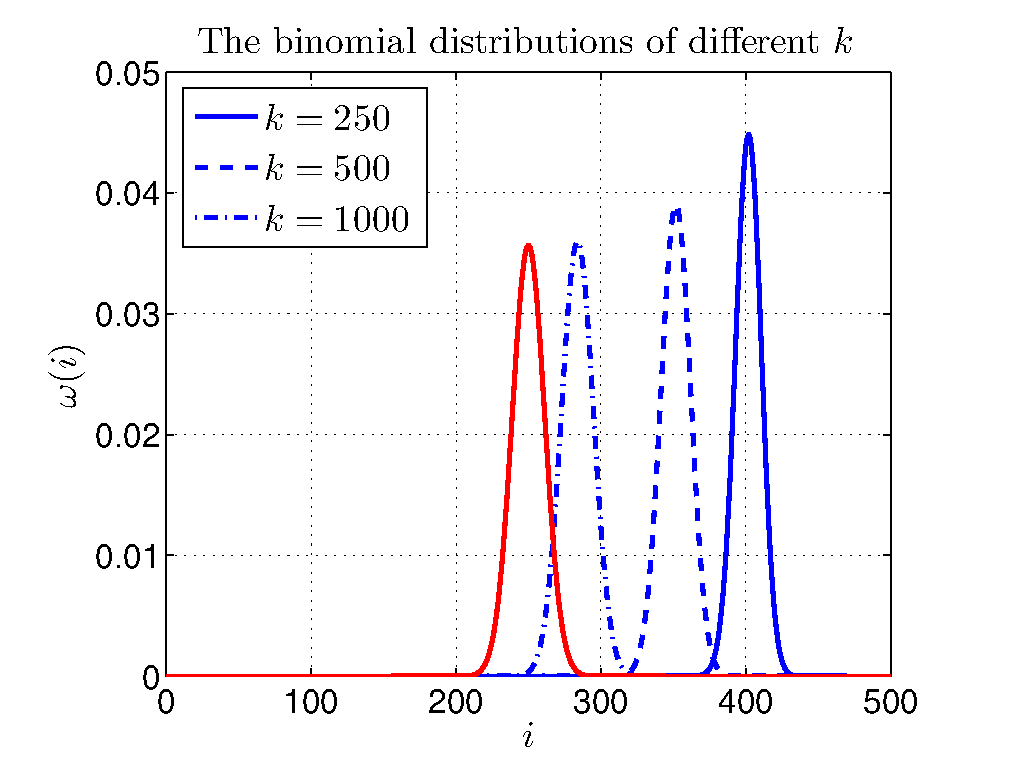
\includegraphics[width=0.40\textwidth,trim=0cm 0cm 0cm 0cm]{deltaMexample2a}}
{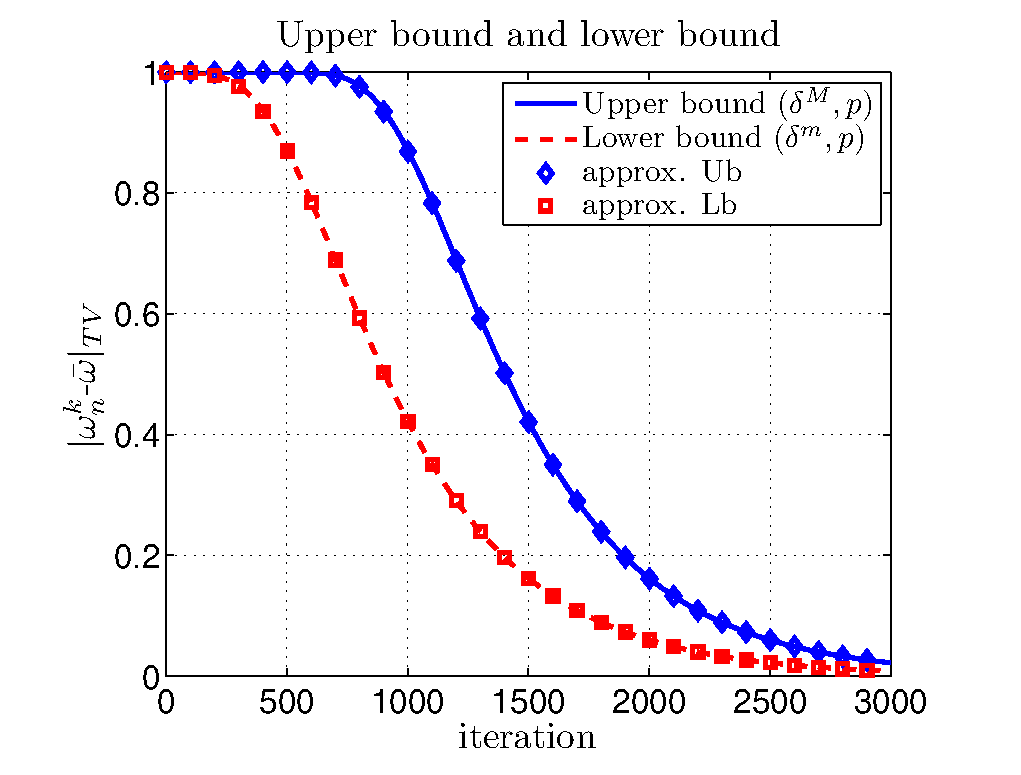
\includegraphics[width=0.40\textwidth,trim=0cm 0cm 0cm 0cm]{deltaMexample2b}} %\\
\end{tabular}
}
\centerline{
{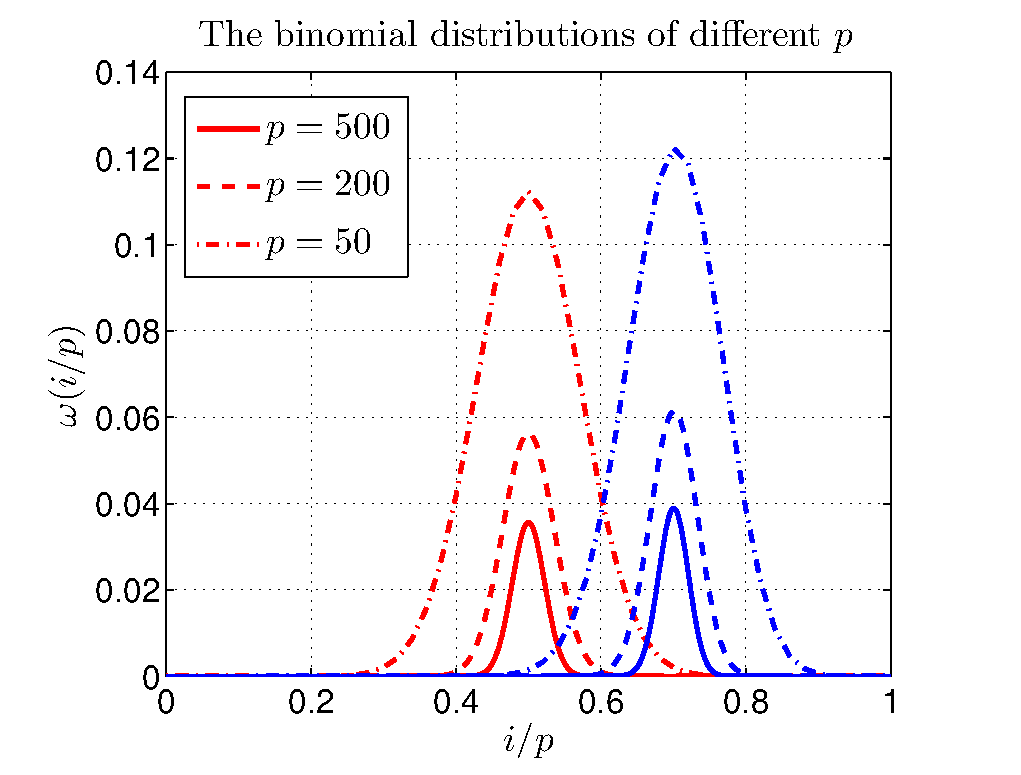
\includegraphics[width=0.40\textwidth,trim=0cm 0cm 0cm 0cm]{deltaMexample1a}}
{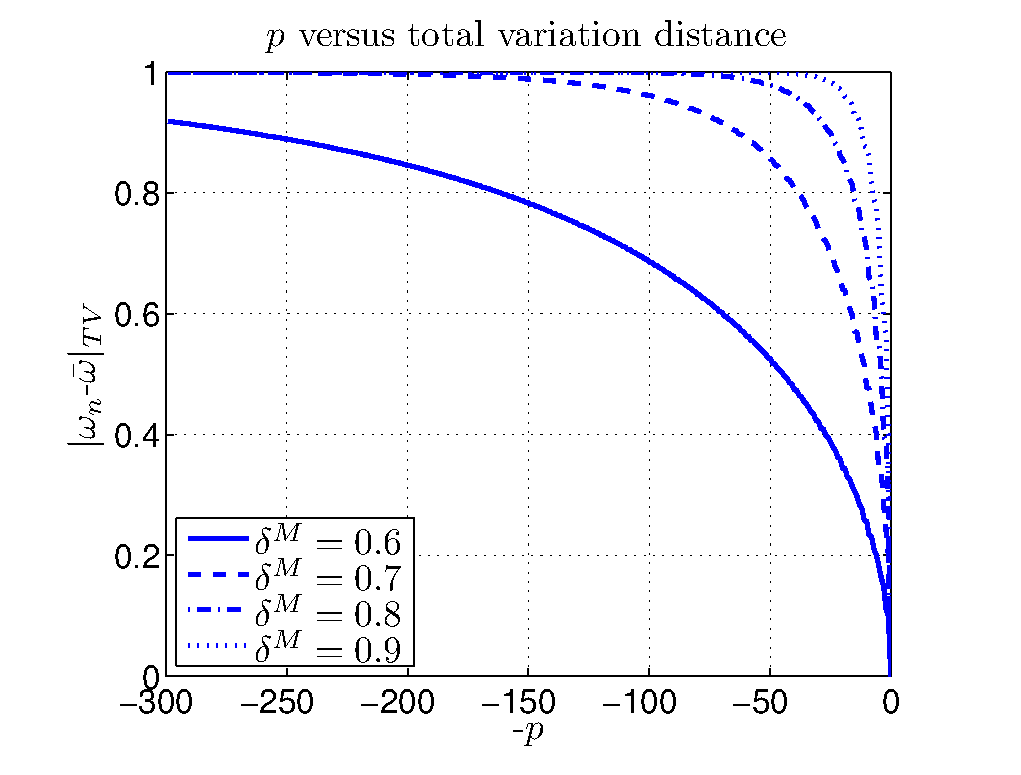
\includegraphics[width=0.40\textwidth,trim=0cm 0cm 0cm 0cm]{deltaMexample1b}}
}

\end{frame}



\end{document}
